\documentclass[sigplan,twocolumn,review,anonymous]{acmart}
\renewcommand\footnotetextcopyrightpermission[1]{}
\pagestyle{plain}
\settopmatter{printfolios=true,printacmref=false}
\acmSubmissionID{1123}
\usepackage[utf8]{inputenc}
\usepackage{setspace}
\usepackage{xspace}
\usepackage{listings}
\newboolean{showcomments}
\setboolean{showcomments}{true}
\ifthenelse{\boolean{showcomments}}
{ \newcommand{\mynote}[3]{
    \fbox{\bfseries\sffamily\scriptsize#1}
    {\small$\blacktriangleright$\textsf{\emph{\color{#3}{#2}}}$\blacktriangleleft$}}}
{\newcommand{\mynote}[3]{}}

\usepackage[ruled, vlined, linesnumbered]{algorithm2e}
\usepackage{amsmath, amsfonts, amsthm,microtype}
\usepackage{tablefootnote}
\usepackage{xcolor}
\usepackage{enumitem}
\definecolor{darkgreen}{rgb}{0.0, 0.5, 0.26}

\newcommand{\mm}[1]{\mynote{mm}{#1}{blue}}
\newcommand{\sa}[1]{\mynote{sa}{#1}{orange}}
\newcommand{\pf}[1]{\mynote{pf}{#1}{darkgreen}}
%\newcommand\sa[1]{\textcolor{orange}{\textbf{SA:} #1}}
%\newcommand\pf[1]{\textcolor{darkgreen}{\textbf{PF:} #1}}

\newcommand{\sys}{\textsc{rose}\xspace}
\newcommand{\efibitalic}{\textit{external-fault-induced bugs}\xspace}
\newcommand{\efib}{external-fault-induced bugs\xspace}
\newcommand{\efibshort}{EFIBs\xspace}
\newcommand{\efibsingle}{EFIB\xspace}

\title{OS Level Reproduction of External-Fault-Induced Bugs}
\title{General-Purpose Reproduction of External-Fault-Induced Bugs}
\title{General Reproduction of External-Fault-Induced Bugs}
\title{\sys: Systematic Reproduction of External-Fault-Induced Bugs}
\title{Reproducing External-Fault-Induced Bugs}
\title{\sys: Reproducing External-Fault-Induced Bugs}
\title{\sys: Reproducing External-Fault-Induced Failures in Distributed Systems with Lightweight Instrumentation}

%\title{Reproducible Fault Injection at the OS Level}
\author{Sebastião Amaro}
\affiliation{
  \institution{IST Lisbon \& INESC-ID}
  \country{Lisbon, Portugal}
}
\author{Miguel Matos}
\affiliation{
  \institution{IST Lisbon \& INESC-ID}
  \country{Lisbon, Portugal}
}
\author{Pedro Fonseca}
\affiliation{
  \institution{Purdue University}
  \country{West Lafayette, Indiana, U.S.A}
}

\newcommand{\mypara}[1]{\noindent{\bf {#1}~}} 
\acmConference{}{}

\lstdefinestyle{yaml}{
    basicstyle=\ttfamily\footnotesize,
    keywordstyle=[1]\color{blue}\bfseries,
    keywords=[1]{execution_plan, setup, workload, nodes, faults, block_ips, process_restart,process_restart2, begin_cond, condition},
    keywordstyle=[2]\color{teal}\bfseries,
    keywords=[2]{script, duration, container, binary, ip, leader, type, time, binary_loc, symbol, offset, call_count, ips_in, ips_out,target},
    commentstyle=\color{gray},
    stringstyle=\color{red},
    showstringspaces=false,
    breaklines=true,
    frame=single,
    rulecolor=\color{lightgray},
    tabsize=1
}

\begin{document}
\begin{singlespace}
\begin{abstract}
Distributed systems form the backbone of critical infrastructures, yet remain vulnerable to \emph{external-fault-induced bugs} that manifest only when specific external events occur during specific application states. 
Existing approaches to reproducing these bugs require fine-grained information about the application, which might not be available in production, and operate within a limited fault model.
\sys is a novel black-box approach that collects traces from production environments and systematically generates fault schedules that reproduce these bugs.
By leveraging the insight that external faults are observable through system interfaces, \sys uses lightweight tracing (2.6\% overhead) to capture essential system-environment interactions.
Then, it identifies the application states when faults must occur to trigger bugs, and generates schedules that consistently reproduce these bugs.
\sys successfully reproduced 20 bugs across eight production systems implemented in diverse languages (C, C++, Java, Go, Scala), including widely-used systems such as Zookeeper, MongoDB, and HBase.
\end{abstract}

\maketitle

% Automatic reproduction of external-fault-induced bugs
% Rose: Leveraging the environment to reproduce extern-fault induced bugs
% Rose: automatic reproduction of external-fault induced bugs
% What? When? How? Diagnose! Reproduce! An agnostic approach to external-fault-induced bugs
% Rose: OS-level Fault Injection for reproduction
\section{Introduction}

%\pf{We need to think a bit more about the title of the paper.}
%\sa{Thinking of possibilities.}
%\pf{Double check that the template is well configured.}
%\sa{Checked.}
Distributed systems underpin critical infrastructure services, and their failures can result in substantial revenue losses and service disruptions~\cite{googleoutage, spotifyoutage, openaioutage}.
Despite advances in, and adoption of, formally proven algorithms~\cite{tla+microsoft} and fault tolerance mechanisms~\cite{avizienis2001fundamental,bft_survey}, widely used distributed system implementations remain vulnerable to failures due to software bugs~\cite{bugsIT} that incorrectly handle hardware and network faults~\cite{incidents1,incidents2}.

In this paper we focus on \efibitalic (\efibshort) --- software defects that manifest only when unexpected external events, such as network partitions, disk errors or OS errors, trigger erroneous program states that lead to failures.
Unlike typical bugs that are triggered with specific user input, \efibshort often involve defects in the error handling logic of distributed systems, which is particularly complex, hard to validate in deployment, and difficult to test during development due to the myriad of corner cases.


External faults are outside of the program control.
Systems employ mechanisms to gracefully handle these faults and continue their normal execution correctly.
However, when these faults occur in a specific order and/or in a specific system state they might reveal implementation defects --- we call these defects \efibshort.
%which are only triggered if those sequences and/or conditions are met, we call these \efib.
These factors make analyzing and understanding these bugs extremely hard, and few techniques exist to help developers fix them.
%\pf{I made some changes, but it still needs a pass (reduce redundancy).}\pf{Should fix be the focus of the ending of this last paragraph?}


%\pf{This definition should be clearer ("external" is not defined) and better motivated, i.e., why are we targeting these bugs specifically? Also, I'm not sure the term "fault-induced bugs" is a good one for us (e.g., every bug is caused by a software fault according to the terminology I typically see; see the link I added below). }
% PF: https://ece.uwaterloo.ca/~agurfink/stqam.w20/assets/pdf/W01P2-FaultErrorFailure.pdf
%\pf{The paragraph needs to be better integrated into the text, but it might be easier to figure out how to do this once we have the motivation for focusing on these bugs.}
%\pf{We should try to quantify this class of bugs. }
%\mm{we should also provide the usual definitions of fault/error/failure to avoid any misunderstanding}
%Fault-induced bugs are both prevalent and pernicious, and finding, reproducing and fixing them is a challenging task.
%when they occur in production developers must undertake the task of reproducing them to identify root causes and implement the proper fixes.
%This reproduction task is extremely challenging, with some studies reporting that \textit{“developers spend a vast majority of the resolution time (69\%) on reproducing the failure”}~\cite{pensieve}.

%Many techniques aim to find bugs in distributed systems through fault injection. 
Tools like Jepsen~\cite{jepsen}, Mallory~\cite{mallory} PACE~\cite{AlagappanEtAl16-OSDI}, Chronos~\cite{chronos}, Sieve~\cite{sieve}, FCatch~\cite{fcatch}, and CrashMonkey~\cite{crashmonkey18mohan} employ various strategies to discover bugs by injecting faults and observing system behavior.
Nonetheless, in practice these techniques can not find all bugs due to the massive faults and input search space, and hence many critical bugs still find their way into production leading to production failures. 
%\pf{I think we can compress these paragraphs, the last few sentences are no longer needed, and maybe merge it with another one.} Although bug finding is critical, we argue that it represents only one aspect of improving systems reliability. 
%\pf{We should be more explicit about why are our approach is orthogonal to bug finding: e.g., bug finding struggles to explore the full testing space and in practice critical bugs slip past testing processes and find their way into production code.}
%\sa{Added.}
%\pf{I removed the last sentence. I don't think it was helping. Please check.}\sa{Agree.}
%After a bug is discovered, developers still face the challenging task of reproducing the bug to identify its root cause and implement a solution.

Thus, the ability to reproduce production failures is key to identifying and fixing these bugs.
Unfortunately, this is a complex, time-consuming, challenging process for developers, that often involves manual and ad-hoc approaches, such as manual inspection of logs and code with repeated experimentation of possible fixes.
%Thus, failure reproduction is key to diagnosing production failures and fixing the underlying bugs, but it is a complex, time-consuming, challenging process for developers, and a task that state-of-the-art has failed to address.
As previous work has shown, \textit{“developers spend a vast majority of the resolution time (69\%) on reproducing the failure”}~\cite{pensieve}. 

Bug finding and reproduction are two distinct tasks, with their specific challenges.
Whereas bug finding typically involves exploring a large fault space to uncover potential issues, failure reproduction requires precisely recreating the specific \emph{context} that triggered a bug.
The challenge in reproducing \efibshort is particularly significant for production failures, because tight overhead constraints in production systems limit the information that can be recorded and used, and the complex interplay between system state and fault timing makes failure reproduction extremely difficult.

State-of-the-art works leverage system-specific internals to reproduce fault-induced failures in testing environments.
Pensieve~\cite{pensieve} reconstructs the inputs and steps that led to a failure from log files, while Anduril~\cite{anduril} mimics the occurrence of faults by injecting exceptions at specific points of the execution.
While effective, they are limited to JVM-based deployments since they leverage specifics about Java and the JVM to direct their approaches.
Furthermore, they require fine-grained logs which might not always be available.
%is a time-consuming and complex task for distributed system developers.
%Thus, developers need effective reproduction tools that assist them in diagnosing critical bugs when they are triggered in production with low overhead. 
%\pf{Sebastiao, try to pay closer attention to the topic sentences. Several of them can be more useful, e.g., by making them more specific/complete. }\sa{Attempt at a merge.}
%Bug finding and reproduction are two different tasks with different challenges.


The tension between available information and failure reproduction in distributed systems creates a fundamental challenge. 
Collecting comprehensive runtime information simplifies bug reproduction but entails high overheads for production environments.
As an example, record and replay approaches~\cite{r2,ireplayer,doubleplay,mozilarr} capture all non-deterministic behavior, such as program inputs and thread interleavings.
While these can help reproduce \efibshort during testing runs, they are inapplicable in production given their prohibitive overheads (e.g., RR~\cite{mozilarr} has a minimum overhead of 1.49$\times$). 


To address this challenge, we leverage the insight that only a subset of environment information is often relevant for a given failure.
Furthermore, key interactions between the program and the environment can be recorded with low overhead, potentially allowing the inference of sufficient context to inject the faults that induce \efibshort. 

%To this end, this paper introduces the design of a novel black-box approach that automatically reproduces \efib across diverse distributed systems regardless of system-internals.
To this end, this paper introduces a novel black-box approach that automatically reproduces \efibshort across diverse distributed systems without application-specific annotations or knowledge.
%\mm{commented the external observability principle, I could not get it to fit into the flow without talking about monitoring and fault injection at the same time. Can be added back}
%While internal application state is complex, \efibshort, by definition only affect system behavior when externalized through well-defined interfaces. 
Since the interactions with the environment typically happen through well-defined system interfaces (primarily system calls) \sys strategically monitors system call boundaries to capture the essential contextual information required for bug reproduction with minimal overhead.
%Since \efibshort are caused by external events, 
%We leverage external observability since it suffices for most \efib, since these are caused by external events, we can identify and contextualize them by observing system externals. 
%While internal application state is complex, faults only affect system behavior when externalized through well-defined interfaces (i.e., system calls).
%By monitoring these interfaces, we can capture the essential behavior needed for reproduction with minimal overhead.
%or or to use specific kernel modules.

Realizing this approach requires addressing two key research challenges.
First, given a system trace leading to a bug, we must find \emph{what} faults occurred, and \emph{when} they happened relative to the system execution.
For instance, certain faults are mostly innocuous unless they happen when the system is executing specific functions (see \S\ref{sec:motivation} for a concrete motivating example).  
%\pf{May need to explain better this concept of "relative to the system state", it might not be obvious to everyone what we have in mind.}\sa{Adressed.}
\pf{Still think the definition could be improved, perhaps by making it more formal too. E.g., "conditions the system was in" is still vague. Something like: a preposition on the system state that X. Also, is it really just a condition on the system state (i.e., memory of the program) or is it more of a TLA-style condition, i.e., a temporal condition. Because this is so central to our work, I think we need to do a really good job at nailing down the meaning of this concept.}
This requires distinguishing between normal operation failures (which are expected and handled) and the specific fault sequence that triggered the bug.
We identify common and anomalous events by comparing the production trace of the buggy execution against the trace of a fault-free testing run and, through a diagnosis phase, determine the precise conditions necessary for bug reproduction.

The second challenge involves reproducing production failures in a testing environment. 
After identifying the context that potentially leads to a fault, we need \emph{precise fault injection} mechanisms to inject faults at exact points in the system execution.
Without precision, attempts at reproduction would yield inconsistent results, making the process of finding the correct context impossible.
To solve this challenge, we leverage the insight that external faults only manifest in system behavior at well-defined externalization calls, specifically system calls and network communications.
By injecting faults precisely at these externalization points, we have the control needed for consistent bug reproduction without language-specific instrumentation.

\sys implements this approach using eBPF~\cite{ebpf} to efficiently and safely observe the application, without requiring kernel changes that could hinder production deployments. 

In our evaluation \sys automatically reproduced 20 \efibshort across 8 widely-used production systems written in different languages, namely  HBase (Java), HDFS (Java), Kafka (Java/Scala), MongoDB (C++), RedisRaft (C), Redpanda (C++), Tendermint (Go),  and Zookeeper (Java).
We show that \sys keeps an overhead of 2.6\%, by collecting only partial information about the system and its interactions with the environment.
Finally, we present a discussion on the reproduced bugs, where we delve into what key observations \sys makes to reproduce each bug.


%\pf{This paragraph is out of place. I suggest checking other papers to see how to integrate the related work discussion into the intro.}
%\sa{Moved.}
%\pf{We're missing at least a results paragraph here. Discussing more the implementation could be worth it too. }
%\sa{Adressed.}


%We evaluate it on a collection of bugs, gathered from Jepsen reports, state-of-the-art works, and manual selections.
%This collection contains bugs from different distributed systems written in different languages, and with different goals.
%\sys successfully reproduced 20 bugs, using a trace containing minimal information.

%\pf{This paragraph is out of place. I suggest checking other papers to see how to integrate the related work discussion into the intro.}
%\sa{Moved.}


%\pf{We're missing at least a results paragraph here. Discussing more the implementation could be worth it too. }
%\sa{Adressed.}
 
\paragraph{Contributions.}
This paper makes the following contributions:
\begin{itemize}[leftmargin=*]
    \item A novel black-box approach to reproducing \efibshort in distributed systems.
    %\item \tracer a lightweight tracing system for production environments that captures crucial externally observable behavior with less than 2.5\% overhead per node. \sa{If the \tracer term is gone how do we this contribution?}
    %\item \sys a tool that analyzes a production trace containing a bug, automatically creates precise fault schedules that reliably reproduce bugs, and provides the necessary infrastructure to run them in a testing environment.
    \item The design and implementation of \sys, which contains three components.
    A lightweight tracer designed for production environments that captures crucial externally observable behavior with 2.6\% overhead per node. 
    An analyzer that automatically creates precise fault schedules that reliably reproduce bugs.
    An executor which provides the necessary infrastructure to run schedules in a testing environment.
%    \item An extensive evaluation demonstrating the effectiveness of our approach by automatically reproducing 20 bugs across 8 different production systems\mm{rever números finais}, including Zookeeper, MongoDB, and others.
    \item An extensive evaluation demonstrating \sys effectiveness in automatically reproducing 20 \efibshort across 8 widely-used systems.
\end{itemize}

\section{Background}
This section provides an overview of the key technologies underpinning our approach, specifically how we record application interactions with the environment, and how we precisely inject faults. To this end, we leverage several features of the Linux kernel.

%\pf{There is too much personal language in this section (e.g., "we", "us", "our").}
%\sa{Adressed.}

%It is through system calls that applications make indirect contact with the environment, by environment we denote all external components such as disk, memory, network, etc. Thus, when an external fault occurs, the application will know of it directly (errno in a system written in C) or indirectly (Java exceptions, Results in Rust) through the result of a system call.
%Therefore, we choose to leverage eBPF and other kernel subsystems, this allow us to emulate most of the possible external faults as well as trace key application/environment changes. Since the only requirement for these subsystems is a Linux kernel our contributions can be used in any system running in a Linux kernel.

%\subsection{Linux Kernel Subsystems for Tracing and Fault Injection}
%To achieve lightweight tracing and precise fault injection, we leverage several Linux kernel subsystems.
%To record how applications interact with their environment and precisely inject faults we leverage several features of the Linux kernel.


\paragraph{eBPF (extended Berkeley Packet Filter)} eBPF enables the execution of custom programs within the Linux kernel in a sandboxed environment without kernel code modifications.
eBPF programs run with high performance (by executing directly in the kernel) and safety (through verification mechanisms that ensure isolation and termination).
We note that the restrictions imposed by the eBPF verifier, such as checking constraining memory accesses, preventing deadlocks, restricting the number of instructions, among others, make developing these programs potentially challenging.

In our approach, eBPF serves two critical purposes:
\begin{itemize}[leftmargin=*]
\item Fault injection, Using \texttt{bpf\_override\_return}~\cite{override} to manipulate system call results and \texttt{bpf\_send\_signal}~\cite{send_signal} to control (e.g.: pause, crash) processes from kernelspace.
\item System tracing, Monitoring both kernel activity (through \texttt{tracepoints}~\cite{ebpftracepoints} and syscall \texttt{probes}~\cite{ksyscall}) and application behavior (via user-function probes~\cite{ebpfuprobes}).
\end{itemize}

\paragraph{XDP (eXpress Data Path)} XDP complements our tracing capabilities by providing a high-performance framework for processing network packets at the earliest point in the networking stack, right after a packet is received by a network interface card (NIC), and before it is passed to the kernel's networking stack.
We use XDP to efficiently monitor network traffic with minimal overhead, capturing communication patterns essential for reproducing network-related faults.
Some NICs allow running XDP programs entirely on the NIC, allowing users to offload their work from the kernel.


\paragraph{TC (Traffic Control)} TC allows precise control over packet transmission, including selectively dropping packets to emulate network partitions and failures.
%:when XDP (which operates only at packet ingress), TC works at ingress and egress points, enabling the creation of diverse fault scenarios.
While XDP  operates only at packet ingress, TC works at ingress and egress points, enabling us to create diverse fault scenarios.

%\mm{podemos terminar com uma frase deste género se houver espaço, deixo comentado para já}
%Together, these technologies provide a comprehensive platform for observing system behavior and injecting faults with high precision at the OS level, enabling language-agnostic bug reproduction with minimal overhead.

\section{A Reproducibility Challenge}
\label{sec:motivation}

To demonstrate the difficulty in reproducing \efibshort, let us consider bug \texttt{RedisRaft-43}~\cite{redisraft43} (detailed in Table~\ref{tab:bugs}, and \S\ref{sec:evaluation}), a real bug discovered by Jepsen~\cite{jepsen} in RedisRaft~\cite{redisraft}, a Redis module implementing the Raft consensus algorithm.
This bug manifests as a node panicking on restart, due to a mismatch between log and snapshot indexes.
Jepsen discovered this bug by randomly injecting a combination of process crashes, pauses, and network partitions.
The only information reported is an error message from a failed assertion that validates these indexes must match.

As a preliminary attempt to try to reproduce this bug, we analyzed the Jepsen test history to extract the sequence of faults injected right before the system crashing.
Next, we manually created a simple schedule incorporating these faults in an attempt to trigger the bug. 
We empirically found that the last three faults (we tried other combinations) before the crash were enough to reproduce the bug, but with a very low success rate (1 in 100 executions), demonstrating the difficulty of manually recreating the precise conditions needed. Some serious bugs are even more difficult to analyze, which explains why some remain unfixed, despite having been triggered in production, for days, weeks, or even months. 
~\cite{pensieve} reports, by studying 30 randomly sampled failures, that the average absolute time until a failure is reproduced is around 79 days (69\% of resolution time).
This scenario highlights two key challenges.
First, random fault injection provides no guarantee the bug will recur in subsequent test runs, making timely debugging impossible. 
Second, error messages alone provide insufficient information to determine \emph{what} fault conditions triggered the bug or \emph{when} they occurred relative to the system state.
Such a low replay rate and scarce information makes it hard for developers to understand the causes of the bug, and time-consuming to test potential fixes.

When we used \sys to analyze the trace from this single successful reproduction, it automatically identified the three critical faults and the specific context in which they needed to occur, generating a schedule that reproduced the bug with 100\% replay rate.
The key insight was that the final fault (a process crash) had to happen when a node was executing a specific function.


%\mm{my proposal is to drop this entirely, we're short in spcae and time and already discuss this at some lenght in the intro}
%\subsection{System Calls and External Observability.}
%\sa{Moved system calls and external observability to Motivation, and removed the first paragraph. I think we do not have to say in a systems conference that system calls are an interface between OS and applications.}\pf{Looks good to me.}
%%System calls serve as the interface between applications and the operating system kernel, providing the means through which applications can access hardware resources and OS services.
%External faults (disk errors, network issues, etc) are typically exposed to applications through the system call interface.
%For example, a disk failure can appear as a system call error when an application attempts I/O operations.
%%\pf{This is not entirely accurate; a disk failure could cause a instruction to not execute, a CPU failure could also cause similar problems. Even data accesses through asynchronous IO, using memory mapped files, could cause an error outside system call invocations. We need to fix this. }
%%\sa{Changed to "substantial" external faults}
%%\pf{Also, what we're sayings here is not background, it's motivation / approach. But I suggest we try to fix the intro first  and then fix this (e.g., we also don't want too much redundancy with the intro)}
%%\sa{Agree, TODO: Moved to approach}
%\pf{Check my change :) }
%
%This observation underpins our approach: by monitoring and manipulating system calls, we can observe and reproduce the external faults that trigger bugs.
%Furthermore, this approach is completely agnostic of the application details since, regardless of implementation language, all applications must use system calls to interact with their environment.

%\pf{My concern with this text is that it makes it sound like this is a big insight, but to me it is a relatively standard way of instrumenting programs or recording program executions.}

\section{\sys}

\sys is designed to help developers reproduce \efibshort that previously occurred in production systems.
It assumes a black-box model that does not require any knowledge of system internals or language-specific instrumentation.
%We start by introducing a real-world bug example to illustrate the challenges of reproducing \efib, and then present how our system design addresses these challenges.

%\section{A Reproducibility Challenge}
\label{sec:motivation}

To demonstrate the difficulty in reproducing \efibshort, let us consider bug \texttt{RedisRaft-43}~\cite{redisraft43} (detailed in Table~\ref{tab:bugs}, and \S\ref{sec:evaluation}), a real bug discovered by Jepsen~\cite{jepsen} in RedisRaft~\cite{redisraft}, a Redis module implementing the Raft consensus algorithm.
This bug manifests as a node panicking on restart, due to a mismatch between log and snapshot indexes.
Jepsen discovered this bug by randomly injecting a combination of process crashes, pauses, and network partitions.
The only information reported is an error message from a failed assertion that validates these indexes must match.

As a preliminary attempt to try to reproduce this bug, we analyzed the Jepsen test history to extract the sequence of faults injected right before the system crashing.
Next, we manually created a simple schedule incorporating these faults in an attempt to trigger the bug. 
We empirically found that the last three faults (we tried other combinations) before the crash were enough to reproduce the bug, but with a very low success rate (1 in 100 executions), demonstrating the difficulty of manually recreating the precise conditions needed. Some serious bugs are even more difficult to analyze, which explains why some remain unfixed, despite having been triggered in production, for days, weeks, or even months. 
~\cite{pensieve} reports, by studying 30 randomly sampled failures, that the average absolute time until a failure is reproduced is around 79 days (69\% of resolution time).
This scenario highlights two key challenges.
First, random fault injection provides no guarantee the bug will recur in subsequent test runs, making timely debugging impossible. 
Second, error messages alone provide insufficient information to determine \emph{what} fault conditions triggered the bug or \emph{when} they occurred relative to the system state.
Such a low replay rate and scarce information makes it hard for developers to understand the causes of the bug, and time-consuming to test potential fixes.

When we used \sys to analyze the trace from this single successful reproduction, it automatically identified the three critical faults and the specific context in which they needed to occur, generating a schedule that reproduced the bug with 100\% replay rate.
The key insight was that the final fault (a process crash) had to happen when a node was executing a specific function.


%\mm{my proposal is to drop this entirely, we're short in spcae and time and already discuss this at some lenght in the intro}
%\subsection{System Calls and External Observability.}
%\sa{Moved system calls and external observability to Motivation, and removed the first paragraph. I think we do not have to say in a systems conference that system calls are an interface between OS and applications.}\pf{Looks good to me.}
%%System calls serve as the interface between applications and the operating system kernel, providing the means through which applications can access hardware resources and OS services.
%External faults (disk errors, network issues, etc) are typically exposed to applications through the system call interface.
%For example, a disk failure can appear as a system call error when an application attempts I/O operations.
%%\pf{This is not entirely accurate; a disk failure could cause a instruction to not execute, a CPU failure could also cause similar problems. Even data accesses through asynchronous IO, using memory mapped files, could cause an error outside system call invocations. We need to fix this. }
%%\sa{Changed to "substantial" external faults}
%%\pf{Also, what we're sayings here is not background, it's motivation / approach. But I suggest we try to fix the intro first  and then fix this (e.g., we also don't want too much redundancy with the intro)}
%%\sa{Agree, TODO: Moved to approach}
%\pf{Check my change :) }
%
%This observation underpins our approach: by monitoring and manipulating system calls, we can observe and reproduce the external faults that trigger bugs.
%Furthermore, this approach is completely agnostic of the application details since, regardless of implementation language, all applications must use system calls to interact with their environment.

%\pf{My concern with this text is that it makes it sound like this is a big insight, but to me it is a relatively standard way of instrumenting programs or recording program executions.}

\sys requires developers to provide the system binaries, a representative workload and a bug oracle.
The workload serves to drive the system during testing and the bug oracle is used to identify the presence of a bug.



\begin{figure*}[htbp]
	\centering
	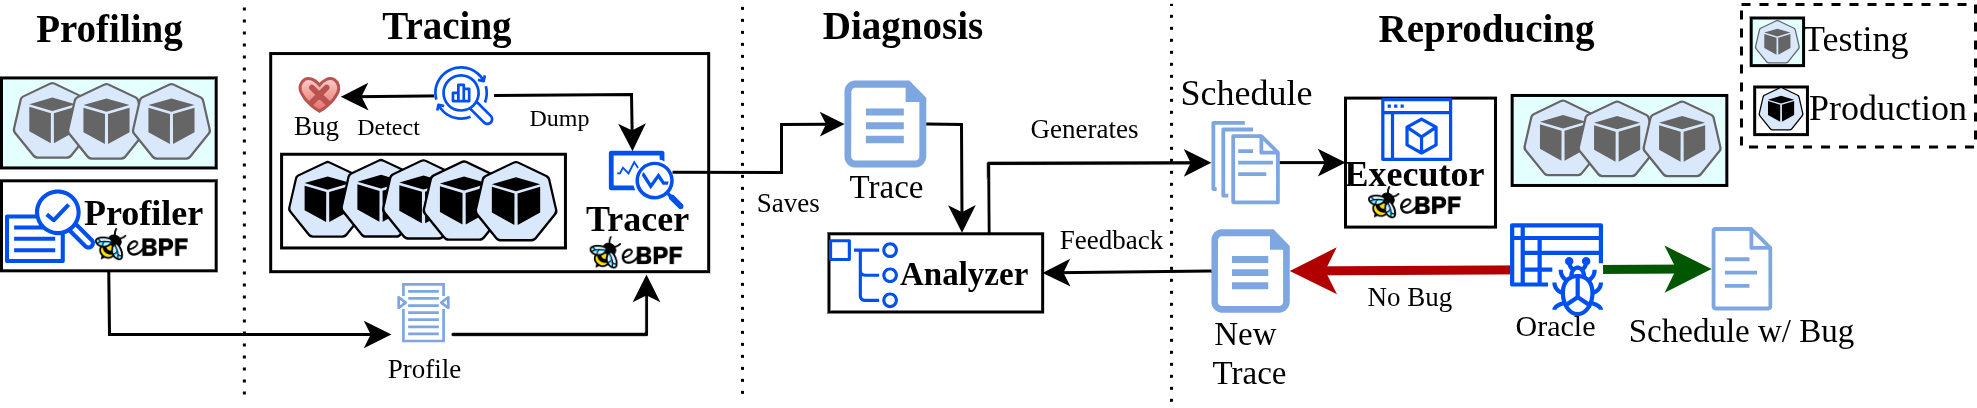
\includegraphics[height=0.16\textheight]{Figures/ROSE-Paper Workflow.png}
	\caption{Workflow of \sys.}
	\label{fig:workflow}
\end{figure*}

\subsection{Target Bugs}
\sa{R2C4,R3C1: New Section }
\label{sec:targetbugs}
In this work, we aim to reproduce \efibshort, these are bugs which are revealed by external faults that occur in the environment.
This is the only condition for \sys to reproduce a bug, the underlying semantics of the bug, recovery, consensus, snapshooting, etc. are not relevant
in this work.
\efibshort that need fine-grained and detailed dataflows are out of our scope, since we do not currently collect information about the inputs and outputs of the system.
If the developer has access to this information, then \sys can reproduce the bug.
\sa{Not sure about adding these lines about data/control}


\subsection{Overview and Workflow}
\label{sec:overview}

To reproduce \efibshort, \sys follows the workflow depicted in Figure~\ref{fig:workflow} which consists of four phases.

\mypara{Profiling phase}. This phase identifies common faults in the system, collects system call frequency, and optionally identifies infrequent functions that might represent important system state changes.

\mypara{Tracing phase.} This phase deploys a production tracer to capture relevant system events.
When a bug occurs, as indicated by the bug oracle, it dumps the trace to disk.

%iii) \emph{diagnosis phase} - analyzes the trace a identify the \emph{fault context}, conditions necessary for a fault for the bug to occur, and produces a fault schedule,
\mypara{Diagnosis phase.} This phase analyzes the trace to identify \emph{fault contexts} that might trigger the bug and generates the corresponding fault schedules.
Fault contexts correspond to sequences of necessary conditions that must be observed before faults are injected.

\mypara{Reproduction phase.} This phase executes the fault schedule and uses the oracle to check whether the bug is reproduced.
If it did not occur, it passes the information collected during the execution to the diagnosis phase, which will use it to gener ate the next fault schedule.
If the bug is found, it repeats the execution multiple times to assess whether this schedule reproduces the bug with a configurable success rate (we used 60\% in our evaluation).
The workflow terminates once a schedule reproduces the bug with the target success rate or if it can not generate more schedules.

%Attempting to reproduce fault-induced bugs in any type of deployed system creates three key challenges: first, we must decide which information we want to gather and what we can gather due to overhead complications. Second, from this collected information, we must find the key aspects of the execution that led to the bug. Third, we must precisely replay the faults that occurred in the deployment.
%\sys addresses these challenges in the following way: it employs low-overhead tracing to deployed systems based on tracing externally observable behavior common to all systems, keeping a batch of the most recent events in the deployment. When a bug occurs, this batch is saved to disk.

%MM: isto depois é um pouco repeteido na discussão, cortei aqui.
%\mm{uniformizar com termos da intro.}
%The profiling and tracing phases address the \emph{information capture} challenge by determining what information to collect from production systems while maintaining low overhead.
%The diagnosis phase addresses the \emph{fault context} challenge by finding the key aspects of execution that led to the bug and the reproduction phase addresses the challenge of \emph{precise fault injection} by accurately replaying the faults in the right context.
%Next, we describe the design of each phase in detail.


%\sys uses this trace to find what faults occurred by looking for unexpected events.
%With a list of faults, we employ an Algorithm that leverages fault specifics and the events that precede them to find the necessary context for the bug to occur. This is accomplished by iteratively creating best-guess schedules, running them, and leveraging the feedback to create a better guess.
%A high-level workflow of \sys is illustrated in Figure~\ref{fig:workflow}. Developers need to provide a system binary, a list of key system files, a way to deploy the system in a controlled environment, a workload, and an oracle to confirm the presence of the bug.


\subsection{Profiling}
\label{sec:profiling}

\sys can reproduce most bugs (15/20 in our evaluation) using only externally observable behavior.
However, for certain bugs, this information is not enough to build a schedule that reproduces the bug with an acceptable rate.
%This is because some bugs only manifest when the system is in specific states, i.e. executing specific application functions.
This is because some bugs only manifest when the system is executing specific application functions.

The goal of this phase is to identify which of these functions might be relevant through a frequency-based heuristic.
Developers provide a list of functions or files that control critical system functionalities (e.g: recovery procedures, leader change mechanisms, snapshotting, etc).
\sys then runs the system with a representative workload in a failure-free testing environment and counts function invocations, separating them into frequent (a configurable value, defaults to 2 calls per second) and infrequent groups.
Frequently called functions are discarded, and the rest are passed as monitoring sites (in addition to the system calls, monitored by default) to the tracing phase.
The intuition is that \efibshort typically involve code paths that rarely execute during normal operation.
This approach maintains our black-box philosophy by working with any system while providing just enough internal state visibility to capture critical execution contexts.
\sa{R1C7,R3C3: While the names of the files are specific information to the system, for \sys they are only addresses/offsets within a binary. Instead of asking developers to give the addresses themselves, which is a general solution, we think that providing the filenames and having \sys collect the addresses is a simpler approach and makes \sys easier to use.}.

Additionally, we also collect information about any faults that might occur since some faults are common even in failure-free executions, as well as the frequency of system calls in the system, to distinguish between common and rare system calls.
This information is latter used to guide the search in the diagnosis phase.

\subsection{Tracing}
\label{sec:tracing}

\mm{num sistema real teríamos que fazer merge de traces de várias máquinas físicas. Qual é a abordeagem para isto?}
\sa{Concatenar os logs e ordernar pelo tempo, abordado.}
In this phase, \sys monitors the target system, keeping a sliding window of recent relevant events (1 million by default), and provides a \texttt{dump} primitive to write the window to disk.
This primitive is externally invoked either manually by an operator or, more typically, by the existing monitoring infrastructure when a deviation from normal behavior is detected.
The tracer runs on each application node.

\subsubsection{Events} We represent the trace as a sequence of events:

\[Trace = \Big( E_i = \{ts,type,I\} \Big)_{i=1...n} \]
where each event $E_i$ is associated with a timestamp $ts$, the $type$ of event, and event specific information $I$.
There are four event types.

%The number of events saved (x) has a default value of 1 million, with this approach, we do not consume extra memory/disk space as a naive save-everything approach would.
%\[Trace = \sum_{n=x}^{y} Event \{id,Context,ts,rt\} \ (4)  \]
%Events in \tracer are represented by their id, which represents the type of event, their context, which details specifics about the event, the timestamp at which they occurred, and their relative time. Context is different for all types of events and gives key information about the event.
%It is by looking at sequences of events and their context that we can find clues about what faults happened, and in what context they occurred. The event with the earliest timestamp will be considered the first one, and the relative time of the others will be calculated accordingly.
\mypara{System Call Failures (SCF).}
The most common event is system call failures (SCF).
Even though SCFs are not uncommon, they provide key insights into the (unsuccessful) interactions between the system and the external environment.
The tracer monitors system calls and when they return an error, we record the process id, the system call id~\cite{syscallids}, the file descriptor(for file-related I/O operations), and the \texttt{errno} return code.
For file-related system calls that use the filename instead of the file descriptors, such as \texttt{open} and \texttt{stat}, we capture the filename.
The filename allows us to have a richer context about the possible problematic event, and the \texttt{errno} allows us to later replay and emulate this event.
\[ SCF_I = \{pid, syscall\_id, fd,filename, errno\}  \]

%These failures often indicate external faults (network issues, disk errors) affecting the system.
%The base context for these events is: the pid, the errno return code, and a filename if the system call is related to I/O or other operations on files (e.g. stat). The pid allows us to identify the node, the ID allows us to identify the system call,

%When a node in a production distributed system has a buggy behavior it is revealed to others through system calls. Many incorrect internal mechanisms can happen, but barring the process crashing, being isolated from the network, or stopping, it is when another node makes contact with it that this incorrect state will reveal itself. The same insight applies to application state changes, when a node has a relevant state change, such as going from follower to leader, it is only at the point at which this change becomes external that it becomes known to the overall system.


\mypara{Application Functions (AF).}\label{userfunc}
The tracer also captures the infrequent function invocations, capturing important information about application state changes.
We record the process id and a function id, a unique integer associated with each function defined during the profiling phase.
\[ AF_I = \{pid, function\_id\}  \]

%Note that to keep tracing as lightweight as possible we do not capture any further information about the function such as function parameters.
%We will further discuss the impact of this in \S\ref{sec:diagnosis}.


\mypara{Network Delays (ND).}\label{networktracing}
Network partitions and failures are a common cause of \efibshort.
Network failures capture a wide-range of general behaviors such as packet loss, link flapping, or latency spikes, among others, while network partitions capture specific failure patterns where the system is split into two or more subsets of nodes: nodes are able to communicate with other nodes within the subset but not with nodes in other subsets (either in one or both directions).

While some network failures can be captured as system call failures (e.g.: a \texttt{connect} failure) others cannot (e.g.: latency spikes).
Temporary network partitions/failures also pose a problem --- while, for instance, a failed \texttt{connect} might indicate the beginning of a network partition, since we do not track successful system calls we are not able to detect when the partition is healed.
We therefore need a more robust method of detecting network issues and their duration.

Since periods of network inactivity may indicate partitions or connectivity issues, we employ a strategy that aims to detect network delays (ND) as a proxy for identifying possible network failures or partitions.
We detect these delays by keeping a map of active connections.
When a node sends a packet, we calculate the delay between this packet and the last time a packet was sent in this connection.
If the delay is longer than configurable value (5 seconds by default), we record a network delay event, containing the source and destination IPs, the duration, and the number of packets sent in the connection up until this moment.
\[ND_I = \{Dest\_IP , Source\_IP , Duration, Packet\_Count\}  \]


\mypara{Process States and Restarts (PS).}
Process crashes and pauses are other common source of \efibshort where the crash/pause of a process triggers a cascading effect in the rest of the system.
We monitor this by keeping track of the process state --- if a process is in the \texttt{waiting} state for more than a configurable time (3 seconds by default), we record this as a possible fault.
We also create an event when a  process crashes.
We record the process id, the state of the process, and for process pauses, the duration of the pause.
%Processes crashes can be detected by the above solution, however, a restart can not. This is because when an application node starts again, it is assigned a new pid, which the tracer is not aware of. We ask developers to provide information about the node when it reboots to the tracer, so the tracer can create the necessary infrastructure to trace this new process. This is a simple write to a file with application node name, and pid.
\[PS_I = \{pid, State, Duration\}  \]
%\mm{como é que a duração é medida se um processo tiver 9 secs em waiting? são 3 eventos de duração 3? ou 1 evento de duração 9? o State é apenas waiting? Ou crashed? O restart é também um state?} \sa{Mais que 3 segundos, corrigido no texto}
%\mm{mas se a falha demoara 9 segundos quantos events ~são gerados? 1 com Duration=12 ou 4 com Duration=3?}\sa{Duration=9}
%MM a consequência disto é que se a pausa continuar e se fizer o dump não vemos esse evento no log. Deveríamos ter uma forma mais sistemática de lidar com isto, por exemplo emitindo eventos pendentes quando se faz dump.

%\mm{comentei a parte do restart acim{mas se a falha demoara 9 segundos quantos events ~são gerados? 1 com Duration=12 ou 4 com Duration=3?}, acho que pode ir para a impl. pois creio que isso poderia ser automatizado sem ter que pedir info extra ao utilizador, podemos disctuir depois}


\mypara{Event Duration.}
For events that happen over a time interval, namely network partitions or process pauses, we record their duration and add a single event to the window.
This minimizes the number of events, but also implies that we have to be careful when handling events that did yet terminate when a \texttt{dump} is requested.
For process pauses, if there are ongoing pauses, we save them to the trace.
For network partitions, we check the delay between the last seen packet and the current timestamp and add it to the trace if it surpasses the configured delay for detecting network partitions.

%The trace is then passed to the \emph{diagnosis Phase} which we discuss next. If deployed on multiple machines, we first concatenate the different traces according to their timestamps.
If the tracer is deployed on multiple nodes, we first merge the traces before passing them to the next phase.
%(\S\ref{sec:diagnosis}) which analyzes the events, iteratively refines the execution context, and outputs fault schedules.


\subsection{Diagnosis}

\begin{figure*}[htbp]
	\centering
	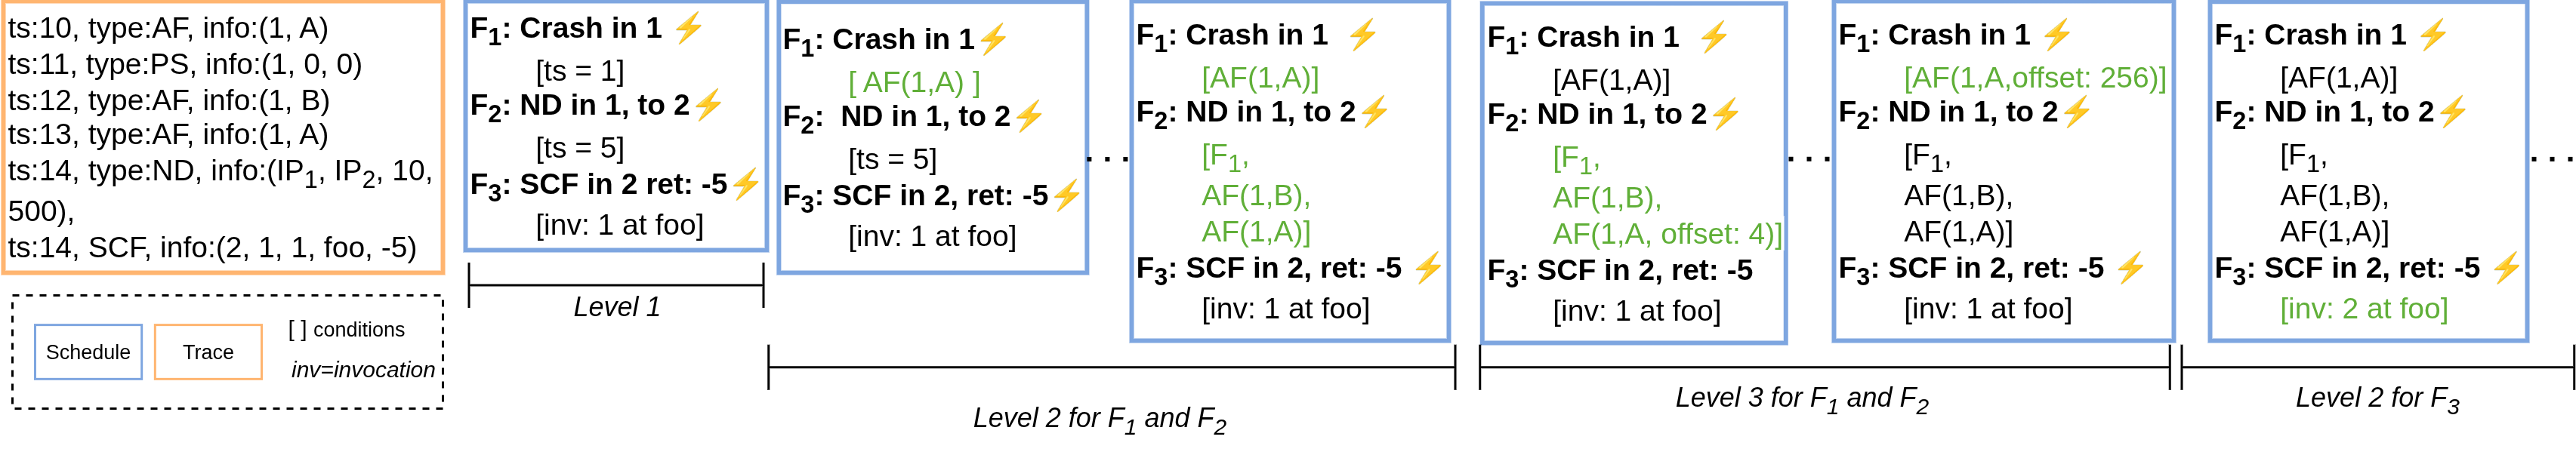
\includegraphics[height=0.135\textheight]{Figures/ROSE-Levels.png}
	\caption{Diagnosis Phase.}
	\label{fig:levels}
\end{figure*}


\label{sec:diagnosis}
The goal of this phase is to identify the necessary \emph{fault context} in which faults should occur, and output a \emph{fault schedule} that reproduces the \efibsingle .
We define \emph{fault context} as the sequence of necessary conditions that must be observed before a fault is injected.
These conditions might include invocation of application-specific functions (AF), particular process states (PS) and network delays (ND), and other system call failures (SCF).
Note that we do not aim to perform root cause analysis and pinpoint the root of the \efibsingle, but instead to quickly create a fault schedule that triggers the bug with a high replay rate.
This creates tension between precision (capturing the right conditions) and relevance (creating a minimal schedule that consistently triggers the bug).

To this end, we employ an iterative algorithm that starts with a basic context (the information of the faults themselves) and iteratively contextualizes each fault, with either the AF events that preceded it, or in the case of SCF, different invocations.
For every iteration, the algorithm outputs a schedule that is passed to the next phase for execution.
If the schedule triggers the bug with a configurable replay rate, we stop, otherwise we refine the schedule based on the execution feedback and try again.
The algorithm builds the fault context in three different levels, as depicted in Figure~\ref{fig:levels}.


\subsubsection{Level 1: Initial Guess.}
\label{sec:levelone}
The algorithm starts by collecting all the faults in the trace.
\sa{R2C1: However, we can not iterate through all the benign faults (faults which do not cause a bug in a system), as this would be an unfeasible task. Thus, we compare a normal execution with the buggy trace obtained from production to discard benign faults.}
\sa{Should I give examples of this here, or in the evaluation?}
Given this set of faults, the challenge is how to select which ones to contextualize first, to create a schedule within an acceptable time.
We prioritize faults based on their potential impact on the system and their expected frequency, with less frequent faults having more priority, as well as faults that are in the trace but have not been observed during the profiling phase.
In detail, we prioritize first PS, then ND and finally SCF, and within each category we follow chronological order.
The rationale is that later faults might be due to earlier faults and hence be a symptom rather than a cause.

The algorithm then traverses the sorted list of faults, creating a fault schedule without context and only including the faults' information (fault order, inputs for system calls).

The key insight is that some bugs do not need a particularly complex application state and can be revealed by simply injecting the faults in the correct order.

As an example, for bug \texttt{ZOOKEEPER-3006} (Table~\ref{tab:bugs}), injecting a SCF when opening the snapshot file was enough to reveal the bug.
For SCF we inject the fault by manipulating the error code.
For PS we crash or pause the process for the relevant time.
For ND we inject the respective fault for the duration observed in the trace.
Despite its simplicity, this level quickly identifies \efibshort with straightforward trigger conditions and can create a schedule with 100\% replay rate for 10/20 bugs (Table~\ref{tab:bugs}).

\subsubsection{Level 2: What happened before?}
\label{sec:leveltwo}
If Level 1 fails, we expand the context by triggering the faults at different application states, considering application-specific functions as illustrated in Figure~\ref{fig:levels}.

\mypara{System calls.}
To contextualize system calls where we have input information (e.g.: the filename), we generate schedules that fail the system call at different invocation counts.
As an example this could be failing the first write to a given file, then in the next schedule the second write, and so on.
For system calls where we do not have inputs, we attempt to fail the system call the number of times it appeared in the profiling trace, with a hard cap of attempts (50 by default).
As an example, bug \texttt{HDFS-15032} (Table~\ref{tab:bugs}) is triggered 100\% of the times by injecting a fault in a specific \texttt{connect} invocation.

\mypara{Process and Network faults.} Since these faults do not have context information other than their timestamp and duration, we use previous invocations of AF as context.
The procedure is depicted in Algorithm~\ref{alg:context} and is based on the insight that faults trigger specific code paths to handle them.

\newcommand{\schedule}{$S$}
\newcommand{\fault}{$F$}
\newcommand{\node}{$N$}
\newcommand{\context}{$L$}
\newcommand{\functions}{$AF$}
\newcommand{\runschedule}[1]{\texttt{runSchedule}(#1)}
\newcommand{\oracle}[1]{\texttt{oracle}(#1)}
\newcommand{\confirmbug}[1]{\texttt{confirmBug}(#1)}
\newcommand{\processtrace}[1]{\texttt{processTrace}(#1)}
\SetKwComment{Comment}{$~\triangleright~$}{}
\DontPrintSemicolon
\SetCommentSty{textsf}
\SetKwComment{Comment}{$~\triangleright~$}{}
\SetKwProg{Fn}{fn}{}{end}
\SetKwProg{Upon}{upon}{}{end}
\SetKwIF{If}{ElseIf}{Else}{if}{then}{elif}{else}{endif}
\SetKw{is}{is}
\newcommand{\Update}{\texttt{UpdateShadowPM}()}
\begin{algorithm}[t]
	\scriptsize
	\caption{Context Creation for Process Faults and Network Faults}\label{alg:context}
	% \linespread{1.10}
	\schedule\Comment{Schedule after Level 1 is Executed}
	\fault\Comment{Fault we are creating the Context for}
	\node\Comment{Node where the fault occured}
	\functions\Comment{Functions called by \node which precede \fault~in production trace}
	\context\Comment{List of unique functions to serve as context for F }

	\SetKwFunction{findContextforFaultfn}{findContextforFault}
	\newcommand{\clr}{cacheline\_reords}
	\newcommand{\getcachelinereords}[1]{\texttt{GetCachelineReorderings}(#1)}
	\newcommand{\apply}[1]{\texttt{ApplyState}(#1)}
	\Fn{\findContextforFaultfn{\schedule,\fault,\node,\functions}}{
		\context $\leftarrow \varnothing$\;
		\For{$f~in$ \functions}{
			\lIf{$f~in$ \context}{
				\Return{\context}
			}
			\schedule[\fault] $\leftarrow$  \schedule[\fault] $+$ $f$\;
			$trace \leftarrow $ \runschedule{\schedule}\;
			$bug \leftarrow $ \oracle{} \;
			\If{$bug$}{
				$replayrate \leftarrow$ \confirmbug{\schedule} \;
				\lIf{$replayrate > 60$}{ \Return{\schedule}}
			}
			$(correctOrder,faultInjected) \leftarrow $ \processtrace{$trace$}\;
			\If{$correctOrder~\&~faultInjected$}{
				\context $\leftarrow$ \context $+ f$ \;
				$continue$
			}
			\schedule[\fault] $\leftarrow$
			\lElse{ \Return{\context} }
		}
	}

	\SetKwFunction{confirmbugfn}{confirmBug}
	\Fn{\confirmbugfn{\schedule}}{
	$bugRuns \leftarrow 0$ \;
	$correctRuns \leftarrow 0$ \;
	\For{$run~in [0:10]$}{
	\Comment{If we can not reach our standard rate we leave}
	\lIf{$correctRuns > 3$}{\Return{$0$}}
	$run(S)$\;
	$bug \leftarrow$ \oracle{}\;
	\lIf{ $bug$}{ $bugRuns+=1$}
	\lElse{ $correctRuns+=1$}
	}
	{ \Return{$(bugRuns/10)*100$} }
	}

	\SetKwFunction{processtracefn}{processTrace}
	\Fn{\processtracefn{$trace$,\fault,\functions$Original$,$SsizeL$}}{
		$AF\_trace \leftarrow $ $get\_AF(trace,F)$\;
		\Comment{Compare behavior in production and caused by schedule}
		$correctOrder \leftarrow $ $AF\_trace[0:sizeL]$ == \functions$Original[0:sizeL]$\;
		$faultInjected \leftarrow$ \fault~$in$ $trace$ \;
		\Return{$(correctOrder,faultInjected)$}

	}
\end{algorithm}


We denote faults with $F$ and functions with $f$.
For a given fault $F$, observed on node $N$, the goal is to create a list of unique functions ($L$) to serve as \emph{fault-context} for $F$.
Given the function $f$, that immediately preceded $F$ on $N$, we execute a schedule $S$, where $F$ occurs after $f$ (line 10).
Next, we check for the bug with the provided oracle; if it is present, we confirm if $S$ has the target replay rate (line 14).
If yes, we return $S$ and finish the process, otherwise we continue.
If we observe $L$+$f$ functions in the testing run in the same order as production but the bug is not triggered, it means our sequence is not precise enough to reproduce the bug.
Thus we add $f$ to $L$ (line 18), and move to the next function (line 19).
If we do not observe $f$ in the run, then $F$ is not injected.
This means that $f$ is not likely part of a specific code path to trigger the bug and thus we move to the next fault (line 20).

To generate a new schedule, we search for the function $f+1$ that immediately precedes $f$.
If $f+1$ is not in $L$, we add it to the schedule and execute, repeating the process (line 10).
If $f+1$ is already in the schedule, it means we are no longer in a unique code path, and we move to the next fault (line 9).
The intuition is that functions that occur once are more likely to indicate relevant application-specific states.
\sa{R1C1: While ignoring the duplicate and continuing is a possible option, it would make the algorithm run significantly longer, since \sys would try to construct a context with all the unique functions detected.}

\mypara{Role-specific State.} In many systems, different nodes can assume different roles such as the primary replica in a primary-backup database deployment.
Thus, when a fault occurs, different nodes might show different behaviors contingent on the assumed role.
To handle these scenarios, we employ an \emph{Amplification} heuristic that replicates the schedule across all nodes to determine whether the triggering context is role-specific.
We do \emph{Amplification} if we did not observe $f$ in the testing run.
If $f$ does not appear in any node, it means the context is not role-specific, and we revert this step.
If $f$ appears on some nodes, we leave the schedule as is.
We do not employ this for network faults, since they have consequences on the entire deployment.

%If the fault context is observed in all nodes then this means it is not role specific. \mm{e depois?} Otherwise, we extend the schedule as discussed above and repeat the amplification step.

\mypara{Fault Order.} To faithfully replay what occurred in production we enforce in testing the fault order that was observed in production as detailed in \S\ref{sec:repr:state}.
%However this causes a problem, for example, in a schedule with Faults $A$ and $B$, with contexts $C_A$ and $C_B$.
%When this schedule is run, there is a possibility that $C_B$ occurs before $C_A$, and therefore, the faults would be injected in the reversed order of what was observed in production.
%We address this by enforcing a order between faults, as detailed in \S\ref{sec:repr:state}.

\mypara{Prunning runs.} During fault contextualization, bugs sometimes manifests below the target replay rate due to either incomplete fault contextualization or imprecise context identification.
To address this variability, when we first detect a bug with fault $F$, we immediately evaluate its replay rate.
If we have already seen it, we save the schedule as a possible candidate, and in the end check the replay rate of all candidates.

As an example, reproducing \texttt{RedisRaft-51} (Table~\ref{tab:bugs}) requires injecting the fault when the leader sends the snapshot to other nodes which is role-specific and hence requires the amplification step.
%thus, this bug requires the right fault schedule with the \emph{Amplification} heuristic.


\subsubsection{Level 3: Function-specific context}
\label{sec:levelthree}
In the previous level, and since we capture only the function invocations without any parameters, the faults are injected at the function return point.
Naturally, this misses the fact that functions can contain multiple execution paths, only some of which might be relevant for triggering and reproducing \efibshort.
This can be the difference between a failed and a successful reproduction.
With this in mind, this level creates more refined schedules that inject faults at specific offsets within the functions that immediately precede each fault.
Rather than testing all offsets in sequence, or at random, we prioritize as follows:
i) call sites to system calls,
ii) call sites to other functions, which can reveal system state changes relevant to the bug, and
iii) the rest of the offsets.

For example, reproducing \texttt{RedisRaft-NEW} requires crashing a node executing a \texttt{write} within a specific function.
This corrupts the snapshot and prevents the node from restarting.

\subsection{Reproduction}
\label{sec:reproducing}

This phase executes the target system with the provided workload in the testing environment and injects the faults specified in the fault schedule.
We assume that the developer can provide a representative workload that is able to exercise the relevant code paths that might trigger the bug.
After each execution, we use the bug oracle to infer whether this schedule triggers the bug or not.
In practice, the oracle can be implemented by parsing logs to look for specific errors, automated tools such as Elle~\cite{elle} that check for invariants over the system state, or health checks performed by the production monitoring system, among others.


If the bug is found, the execution is repeated with the same schedule to confirm whether it is able to reproduce with the target replay rate (60\% by default).
Otherwise, the information collected during the execution is fed back to the diagnosis phase, specifically, the information about injected faults and their contexts (lines 34 and 35 in Algorithm~\ref{alg:context}).

The main component of this phase is an \emph{Executor} which:
i) keeps track of the system state;
ii) evaluates the current system state and determine whether a fault needs to be injected; and
iii) injects the actual fault.

\subsubsection{State Tracking}
\label{sec:repr:state}

Since different nodes are likely to be subject to different faults during a testing run, we start by pre-processing the fault schedule to determine which events apply to which node.
Next, we determine for each node the conditions that should be observed in order to inject a fault.

A condition can be a function call, a system call counter, or a system call counter with specifications about their inputs, e.g. the number of times that \texttt{open} must be called with a specific path.
Finally, to preserve the fault order observed in production, we add as conditions to the fault any previous faults that might appear in the trace.
This prevents premature or out-of-order fault injection and eliminates a source of randomness, contributing to better replay rates.
For example in Figure~\ref{fig:levels}, function $A$ is part of the \emph{fault context} of fault $F_2$, meaning we must observe $A$ after injecting $F_1$ in order to injecting $F_2$.
Otherwise, if we observed $A$ before injecting $F1$, this would cause us to inject $F2$ before $F1$ violating the fault order observed in production.
%Thus, we employ the strategy above to enforce the order we saw in production.


%We also leverage time as a condition, time is not a precise metric of system state, but some faults do not need specific context information. Time also allows us to keep a casual order between faults, which depend on function call counters. If time is present as a condition the other conditions will only be taken into account if time is already set. This allows us to keep a casual order between the faults while also making sure they occur after their chains.


\subsubsection{Fault Injection}
\label{sec:overview:fi}
%When all the conditions are satisfied, the fault is injected exactly at the next event where the fault can be triggered.
%When all but one condition for a fault are satisfied, and we encounter the last one, the fault is executed exactly at that system state.
When we observe the last condition that satisfies the fault context, the fault is immediately injected.
The key concern when injecting faults is ensuring precision, i.e. that faults are injected exactly at the same point in the application state across testing runs.
The low-level mechanisms to inject the faults are tied to eBPF's functionalities and are discussed in more detail in the implementation (\S\ref{sec:implementation}), here we focus only on the high-level design and goals.
To fail system calls, we override the return value with the one described in the fault schedule, and completely skip the logic of the system call.
This emulates a scenario where the system call failed right at the beginning of the invocation.
Since we can not know from the production trace whether the system call completed, we opt not to completely skip their execution and return the error code observed in production.
This decision is based on the fact that skipping a system call is a faulty behavior and by returning an error, we force the system to go into the code paths that handle faults.
For process pauses and crashes, we send a signal from kernel space to the target process which ensures the process is crashed/paused consistently in the same state.
For network faults, we drop packets between the target processes as specified in the schedule to emulate a network delay or a network partition.

\section{Implementation}
\label{sec:implementation}

\sys is written in a combination of C and Rust for the performance-critical components, and Python for the utilities and orchestration between the different steps of the workflow (Figure~\ref{fig:workflow}).


\subsection{Profiler}

The Profiler identifies infrequent application functions through static and dynamic analysis, and collects information about the frequency of system calls.
It receives a binary and a list of source file names.
For static analysis, we use a Python script that employs standard Linux utilities (\texttt{readelf} and \texttt{addr2line}) to extract function symbols and their corresponding binary offsets from the target executables.
We then collect all of the symbols defined in the provided files.
For dynamic analysis, we leverage an extended version of the production tracer that also counts functions and system calls invocation frequency.
The Profiler outputs a file containing function names, binary offsets, and invocation frequency statistics, which guides subsequent tracing operations.

\subsection{Tracer}

The tracer is performance-critical since it runs alongside production systems.
It is implemented using \texttt{libbpf-rs}~\cite{libbpfrs}, a Rust binding for the Linux eBPF C library.
We selected Rust for its memory safety guarantees and performance comparable to C/C++ implementations.
The tracer consists of eBPF programs written in C (as required by the eBPF infrastructure) with a Rust control plane that manages program loading, event collection, and trace persistence.

We maintain a fixed-size circular buffer of recent events (1 million by default) using a \texttt{BPF\_MAP\_ARRAY}.
This approach provides a bounded memory footprint and eliminates continuous disk I/O during normal operation.
The buffer contents are only dumped to disk when triggered by the bug oracle, minimizing the impact in production.

Instead of capturing all system calls, we focus exclusively on failures, which are relatively rare but contain the most valuable information about potential faults.
To achieve this, we leverage eBPF \texttt{sys\_exit} tracepoint, which is called every time a system call returns.
We discard all invocations that did not return an error and save those that do in the circular buffer.
Similarly, we trace only infrequent application functions (identified by the Profiler) rather than all function calls, significantly reducing the number of traced events.
Function calls are traced through eBPF user-function probes.


\mypara{File based system calls.}
For file based system calls, it is important to save the full path they operate on.
Instead of saving the full path for every system call (which would require expensive string copies), we maintain a lightweight mapping of filenames to file descriptors, which is only updated during \texttt{open}, \texttt{close}, and \texttt{dup} operations.
Then, to minimize runtime overhead, we reconstruct the path information for each system call in a post-processing step outside the critical path, after saving the trace to disk.

For system calls that operate directly on path names rather than file descriptors (e.g. \texttt{open}, \texttt{stat} ), we record only the userspace address of the variable containing the path name  in the \texttt{sys\_enter}  tracepoint.
If the system call fails, we collect its contents. This way we avoid unnecessary copy operations.


\mypara{Network delays.}
For network delay detection, we leverage XDP (eXpress Data Path) programs attached directly to network interfaces, enabling packet analysis at the earliest point in the networking stack with near-zero overhead.
\sa{R1C2: XDP only supports attaching to the ingress point in the network device, thus we only detect packets on the receiver side of the network interface. Since we attach to the receiver side, we are not affected by sender side packet retransmissions, which would affect our detection precision.}

\mypara{Process State.}
We use the \texttt{procfs}~\cite{procfs} Rust crate to query the process state at regular intervals (default of 1 second).

These implementation choices enable the tracer to maintain overhead below 2.6\% per node (see \S\ref{sec:evaluation}) while capturing sufficient information for fault reproduction.


\subsection{Analyzer}
\sa{O algoritmo é mais complexo que aquilo, acabei for fazer só para a contextualização da falta, deveria ter feito para tudo?}
The analyzer implements the diagnosis phase and receives the profile, a buggy production trace, the workload, oracle, and the application binary.
It iteratively creates fault schedules in YAML format, which are parsed to create a C program implementing the schedule.

This is passed to the executor which starts the tracer.
After the executor executes the schedule, it runs the oracle to check for the presence of the bug, and collects the trace which is to refine the schedule as per Algorithm~\ref{alg:context}.
The Analyzer does static binary analysis to collect the offsets for the application functions, which are used in the Level 3 analysis.
It accomplishes this by disassembling the binary using \texttt{objdump}, and parsing its contents using \texttt{regex}.

\subsection{Executor}
The executor is implemented in C and leverages the \texttt{libbpf}~\cite{libbpf} framework to load, verify, and attach the eBPF programs.
These eBPF programs are system call probes, kernel probes, and user function probes.

To emulate system call faults, we use the kernel system call probe \textit{bpf\_override\_return} which allows overriding the return value of the probed function.
We selected kernel probes instead of \texttt{tracepoints} because they enable the use of \texttt{bpf\_override\_return} while providing the same level of contextual information (timestamps, input arguments, etc.).
%System calls can be overridden at the entry or exit point, hence, we can emulate scenarios where a system call does not complete and returns an appropriate error code, and where it completes but still returns an error code.

To emulate network faults we use custom \textit{Linux TC} filters.
This is achieved by inspecting the packet headers, checking the source and destination IPs, and dropping the packets according to the details of the fault.

Process faults are implemented with the \textit{bpf\_send\_signal} eBPF helper function.
This helper enables sending signals to a process from kernelspace.
We use this approach instead of relying on userspace signals to ensure that the process state manipulation occurs at precisely the intended execution point before the process leaves kernel mode.

\sa{R1C5: \mypara{Function offset fault injection.} To inject faults in specific offsets within functions, we probe a specific offset within the binary using uprobes. When the address is hit, \sys checks if there are any faults to inject and acts accordingly. }
\mypara{Tracking process ids} As we discussed in \S\ref{sec:reproducing} state tracking and fault injection are done on a per-process basis. Our infrastructure, based on eBPF maps, maps the process id to the faults that will occur on it, and the conditions the node (a specific process id) must reach for the faults to be injected.

Since systems commonly spawn child processes to perform certain tasks, there might be scenarios where it is a child process that reaches the condition previously specified.
To solve this issue, we keep a map of child processes to the parent process in the schedule execution.
The decisions are made according to the initial process id, and the faults are injected in the parent. After we inject a process crash, when the node restarts it will be assigned a new process id, thus breaking the initial mapping we did. Similarly to the above, we map the new process id to the original one to make decisions, and inject faults on the new process id.

%With these implementation decisions, we avoid reorganizing the data structures initial created, an do not have to freeze the entire system, replicate and/or restructure the structures initially created. Thus, we can keep a real-world execution of the system.

%As mentioned in Section~\ref{efficientstatetracking}, relevant system calls are separated from irrelevant ones by a {pid, Condition Number} tuple, as well as faults.
%However, processes can create child processes to run other tasks, this is a common behavior in distributed systems.
%Another challenge is handling process restarts since these cause the pid to change, hence, we need a way to tolerate these changes without stopping the entire system and changing all of the preexisting structures.
%We employ a similar method to child processes and map the new pid to the original one.

\section{Evaluation}
\label{sec:evaluation}

The evaluation aims to answer two main questions:
i) how effective is \sys in automatically reproducing \efib, and
ii) what is the overhead of the tracer.
%(1) Is the amount of information enough to find external faults?
%We will also provide an overview of our context analysis and the context necessary for the bugs to occur.
All the experiments were conducted on a machine with 2x Intel(R) Xeon(R) Gold 5320 CPU @ 2.2GHz (52 cores) with 64GB of RAM running Linux kernel 6.11.1.

In summary, \sys automatically reproduced 20 \efibshort (2 of which were uncovered in the process) from eight production systems implemented in various programming languages.
In detail, we reproduce bugs in consensus systems --- RedisRaft (C) and Tendermint (Go), storage/databases --- HDFS (Java), HBase (Java), MongoDB (C++), coordination services --- Zookeeper (Java), and stream processing/message-broker systems --- Kafka (Java/Scala) and Redpanda (C++).
The tracer component achieves an overhead per node of about $2.6\%$.

\subsection{System Selection and Methodology}
To select the systems and the \efib to reproduce, we relied on Jepsen~\cite{jepsen}, Anduril~\cite{anduril} reports, and a preliminary manual bug search.

Jepsen~\cite{jepsen} is a randomized fault-injection tool that maintains a public database of bugs found.
We studied the Jepsen analysis of the last 4 years using as the selection criteria of \efibshort, quantity and diversity.
In the end, we selected RedisRaft\cite{redisraft,redisraftreport} and Redpanda~\cite{redpanda,redpandareport}.
To obtain the trace, which would come from a production deployment, we execute the target system with our tracer and subject it to Jepsen's faults.
This trace is then fed to \sys following the workflow depicted in Figure~\ref{fig:workflow}.


RedisRaft is an extension of the Redis in-memory key-value store, that aims to offer strict serializability through the Raft consensus algorithm.
From the bugs found by Jepsen, we ruled out bugs that did not depend on external events, for example, manual membership changes, since these are not \efibshort.
We also ignored bugs that required Elle~\cite{elle} a transactional consistency checker databases, which Jepsen uses as a bug oracle.
This main reason to ignore these bugs as due to the long execution time of Elle which needs to analyze the entire transaction history.

From a total 21 bugs, we eliminated 13 which where not \efibshort, and 3 that required Elle as an oracle.
Out of the 5 bugs, we managed to obtain traces that reproduced the bug for 4 of them and were able to automatically reproduce 3.
The bug that \sys did not automatically reproduce is explained by the dependency of another bug also happening~\cite{redisraftreport}.
\texttt{RedisRaft-NEW} and \texttt{RedisRaft-NEW2} were two unreported bugs we uncovered when testing with RedisRaft.

Redpanda is a high-performance, Kafka-compatible streaming data platform designed to handle real-time data processing.
Similarly to the RedisRaft methodology we discard bugs which are not \efibshort however for this system we considered bugs that require Elle to illustrate that \sys can be used with complex oracles.
Jepsen reported 11 bugs (note that bug \#1 and \#3039 in the report are the same), 6 of which are not \efibshort.
Out of the 5 bugs, we managed to obtain traces that trigger the bug for 3 of them, 2 of which we reproduce automatically.
These bugs needed Elle to be revealed, and always occur together due to having the same source defect.
For the bug \sys did not reproduce automatically, this stems from the fact that we were unable to compile the binary with debug information due to outdated/missing dependencies, and hence \sys could not run the Level 3 analysis.
%%We expect this to not be problematic for the developers of the system.

Anduril~\cite{anduril} is a recent system that mimics the occurrence of faults by injecting exceptions in Java-based programs.

The bugs reported by Anduril are reproduced by small unit tests or deployments in a small cluster.
Anduril reports 22 bugs, \sa{R4C2: out of these 22 we encountered problems either running or compiling the system in 8 of them. This leaves us 13 possible bugs, we reproduced 10 of these, only one of these \sys can not reproduce since the bug depends on a Interrupted Exception which is an internal Java exception.
	The bugs which we did not reproduce are of the same nature as the ones we did, they require a precise IOException or for \sys a system call failure. Therefore, they would not add new qualitative knowledge about \sys, and only increment the total number of bugs we reproduced.}
\sa{"Rather than aiming to reproduce all the reported bugs, we targeted bug diversity across different systems." Temos de retirar esta frase para fazer sentido.}
Since we do not have traces from when these bugs occurred in production, we recreate the traces by running the test cases provided by Anduril without the Anduril workflow.

\sa{R1C7,R2C2: \mypara{Developer Inputs.} The necessary inputs to reproduce these bugs were as follows. For the Anduril Bugs, we leveraged the tests, mostly unit-tests, provided by Anduril, these serve as a workload and oracle, since the outcome of the test indicates the bug occurs or not. For the other bugs, we constructed generic-representative workloads, which do generic operations in loop (e.g. insert and read for MongoDB) or used Jepsen, which has a similar approach but with append-only lists.
	For oracles, the oracles we designed collect the logs of the nodes in the deployment and then check for a specific message within the logs indicating the presence of a bug. For the redpanda bugs, since Jepsen has a built-in oracle~\cite{elle} we used it directly.
	For lists of relevant files, we looked into the RedisRaft and Redpanda repositories and looked for code files with names that indicate control functionality, e.g., snapshotting, raft, partition, etc.}


\mypara{Key Takeaways.} Out of the 22 available traces, \sys automatically reproduces 20 bugs, achieving close to full completeness.
For 16/20 bugs, \sys achieves a 100\% replay rate, thus proving it can generate precise fault-schedules which consistently show \efib.
Out of 10/20 bugs \sys finds the necessary schedule at the first attempt, showing it can efficiently find the necessary faults and fault contexts to reproduce \efib.

%\mypara{Proof of concept.} As an initial proof of concept, we looked at GitHub repositories of BFT-based systems, where we found \texttt{Tendermint-5839}.
%\mypara{Related work.} We analyzed the state-of-the-art specifically, Anduril, a work recently published, which aims to reproduce \textit{fault-induced failures}.


\subsection{Bug Reproduction}

\begin{table*}[t!]
	\scriptsize
	\centering
	\begin{tabular}{l|c|l|l|c|c|c|c|l}
		\hline
		\textbf{Bug}                                                                                                                & \textbf{Src} & \textbf{Description}                                                    & \textbf{Faults Inj}                                                     & \textbf{RR(\%)} & \textbf{Sched} & \textbf{\#R} & \textbf{Time (m)} & \textbf{FR\%} \\ \hline
		RedisRaft-42~\cite{redisraft42}                                                                                             & J            & Node crashes due to failed assert related to snapshot \& log integrity. & PS(Crash)                                                               & 100             & 1              & 11           & 22                & 60            \\ \hline
		RedisRaft-43~\cite{redisraft43}                                                                                             & J            & Snapshot index mismatch.                                                & \begin{tabular}[c]{@{}l@{}}PS(Crash)*3\\  + ND + PS(Crash)\end{tabular} & 100             & 19             & 29           & 58                & 11            \\ \hline
		RedisRaft-51~\cite{redisraft51}                                                                                             & J            & Node crashes due to failed assert related to cache index integrity.     & PS(Pause)*3                                                             & 90$\pm$8        & 10$\pm$1       & 28$\pm$4     & 56$\pm$7          & 7             \\ \hline
		RedisRaft-NEW~\cite{redisraftnew}                                                                                           & J            & Redis itself crashes due to an inconsistent snapshot file.              & \begin{tabular}[c]{@{}l@{}}ND + \\  PS(Crash) + PS(Crash)\end{tabular}  & 100             & 22             & 32           & 70                & 7             \\ \hline
		RedisRaft-NEW2~\tablefootnote{{This did not show after commit 2d1cf30~\cite{redisraft2d1cf30}, thus we did not report it.}} & J            & Redis itself fails due to a repeated key.                               & ND                                                                      & 100             & 1              & 11           & 11                & 25            \\ \hline
		Redpanda-3003~\cite{redpanda3003}                                                                                           & J            & Redpanda fails to perform deduplication of sent messages                & 5*PS(Pause)                                                             & 70$\pm$14       & 12$\pm$1       & 81$\pm$20    & 324$\pm$82        & 38            \\ \hline
		Redpanda-3039~\cite{redpanda3039}                                                                                           & J            & Inconsistent Offsets                                                    & 5*PS(Pause)                                                             & 70$\pm$14       & 12$\pm$1       & 81$\pm$20    & 324$\pm$82        & 38            \\ \hline
		Zookeeper-2247~\cite{zookeeper2247}                                                                                         & A            & Service becomes unavailable when leader fails to write transaction log. & SCF(write)                                                              & 100             & 5              & 15           & 15                & 80            \\ \hline
		Zookeeper-3006~\cite{zookeeper3006}                                                                                         & A            & Invalid disk file content causes null pointer exception.                & SCF(read)                                                               & 100             & 1              & 11           & 5                 & 60            \\ \hline
		Zookeeper-3157~\cite{zookeeper3157}                                                                                         & A            & Connection loss causes the client to fail.                              & SCF(read)                                                               & 100             & 1              & 11           & 20                & 82            \\\hline
		Zookeeper-4203~\cite{zookeeper4203}                                                                                         & A            & The leader election is stuck forever due to connection error.           & SCF(accept)                                                             & 73$\pm$16       & 16$\pm$3       & 34$\pm$12    & 34$\pm$12         & 83            \\ \hline
		HDFS-4233~\cite{hdfs4233}                                                                                                   & A            & NN keeps serving even after no journals started while rolling edit.     & SCF(openat)                                                             & 100             & 1              & 11           & 11                & 82            \\ \hline
		HDFS-12070~\cite{hdfs12070}                                                                                                 & A            & Files remain open indefinitely if block recovery fails.                 & SCF(fstat)                                                              & 100             & 20             & 30           & 77                & 83            \\ \hline
		HDFS-15032~\cite{hdfs15032}                                                                                                 & A            & Balancer crashes when it fails to contact an unavailable namenode.      & SCF(connect)                                                            & 100             & 26             & 36           & 57                & 91            \\ \hline
		HDFS-16332~\cite{hdfs16332}                                                                                                 & A            & Missing handling of expired block token causes slow read.               & SCF(read)                                                               & 100             & 1              & 11           & 14                & 46            \\ \hline
		Kafka-12508~\cite{kafka12508}                                                                                               & A            & Emit-on-change tables may lose updates on error or restart.             & SCF(openat)                                                             & 100             & 1              & 11           & 22                & 83            \\ \hline
		HBASE-19608~\cite{hbase19608}                                                                                               & A            & Race in MasterRpcServices.getProcedureResult.                           & SCF(openat)                                                             & 100             & 1              & 11           & 11                & 85            \\ \hline
		MongoDB:2.4.3~\cite{mongo-2-4-3}                                                                                            & M            & MongoDB Data Loss Jepsen report.                                        & 2*ND                                                                    & 100             & 1              & 11           & 22                & 16            \\ \hline
		MongoDB:3.2.10~\cite{mongo-3-2-10}                                                                                          & M            & MongoDB Unavailability Jepsen report.                                   & ND                                                                      & 100             & 1              & 11           & 22                & 50            \\ \hline
		Tendermint-5839~\cite{tendermint5839}                                                                                       & M            & Does not validate permissions to access file                            & SCF(openat)                                                             & 100             & 1              & 11           & 5                 & 80            \\ \hline
	\end{tabular}
	\caption{Bugs reproduced by \sys, J=Jepsen,A=Anduril,M=Manual Fault Inj=Faults Injected, R. R=Replay Rate, Sched=Number of Generated Schedules, R\#=Number of runs, Time=Total Time (min), FR=Faults Removed.}
	\label{tab:bugs}
\end{table*}


Table~\ref{tab:bugs} summarizes the \efib automatically reproduced by \sys.
The column \emph{Faults Inj.} reports the faults that had to be injected to uncover the bugs, column \emph{RR (\%)} reports the replay rate, column \emph{Sched.} reports the number of schedules generated before achieving the target replay rate, column \emph{\#R} reports the total number of runs, column \emph{Time (m)} reports the total time taken, \sa{ and \emph{FR} reports the percentage of potential faults for \sys to analyze which are removed by comparing the buggy trace with the trace from a normal execution.}
Recall that after finding a schedule that reproduces the bug, we execute the same schedule ten more times to measure the replay rate.
Hence, in most cases, the number of runs is the number of schedules generated plus ten.
In bugs where \sys can not find all of the key fault contexts, the results may vary. Therefore, for each of these bugs we run \sys 3 times and present the average and standard deviation.

%\sys is able to reproduce a total of 20 bugs in RedisRaft, Redpanda, MongoDB, Zookeeper, HDFS, Kafka, HBase, and Tendermint.
The average number of runs necessary to reproduce a bug with the target replay rate (80\%) is 23, the average number of schedules is 7, and the average execution time is 60 minutes with a standard deviation of 90, mainly due to \texttt{Redpanda-3003} and \texttt{Redpanda-3039}.
Since \sys aims to achieve a high replay rate, it will continue testing schedules until it reaches this goal.
In these two bugs, which in average report a 70\% replay rate lead to \sys running for a longer time.
The longer testing time is also explained by the fact that these two bugs require Elle which takes about 2 minutes to analyze the entire transaction history of each fault schedule.
\sa{In terms of the faults removed by comparing a trace from a normal execution with the buggy trace, we can observe that this comparison allows reducing the search space. In some bugs, it achieves up to 85\% of potential faults removed. As an example: in Java systems it is extremely common for the stat and readlink system calls to fail with a specific error number code, thus by comparing the two traces we can remove these faults as a possible potential fault which revealed the bug.
	While in others it achieves a lesser reduction this is due to the fact that crashes and pauses cause multiple network delays and each individual network delay is a different fault. Since these faults only occurs in the buggy trace they can not be removed.}

The results from Table~\ref{tab:bugs} show that \sys can reproduce fault-induced bugs quickly, and that our diagnosis is effective at automatically deducing the necessary schedule to reproduce bugs.
Due to space constraints we are unable to provide a detailed discussion for all the bugs reproduced, hence we now discuss just a few representative ones.


\mypara{Case study: \texttt{RedisRaft-43}.}
To illustrate \sys diagnostic capabilities, we examine the \texttt{RedisRaft-43} bug (our motivating example in \S\ref{sec:motivation}), where a Jepsen fault sequence achieves only a 1\% replay rate.

\sys starts with the production trace containing the bug and systematically refines the schedule until the target replay rate is achieved.
There are a total of 5 nodes in the system.
The initial \emph{Level 1} analysis (\S\ref{sec:levelone}), considers only basic fault order and produces a schedule that:
i) crash three non-leader nodes,
ii) creates a network partition that isolates the leader, and
iii) crashes the leader.

This schedule fails to consistently reproduce the bug and hence \sys moves to \emph{Level 2} analysis (\S\ref{sec:leveltwo}) which creates the context for each of these faults.
\sys incrementally adds functions to the context (whose invocation must be observed before the fault is injected), eventually identifying that the fault must occur specifically when the \texttt{RaftLogCreate} function is executing, significantly narrowing the fault injection window.
The first thing this function does is call \texttt{prepareLog}, however, since in the Level 2 \sys injects the fault (process crash in this case) right at the beginning of the invocation (function offsets are only explored in \emph{Level 3}), the \texttt{parseLog} function is never run.

The specificity at which exact point in the execution the fault is injected is critical since the bug manifests only when the process is crashed before the invocation of \texttt{parseLog}, and explains the very low reproduction rate of a randomized approach.
With this precisely defined fault context, \sys generated a schedule that reliably achieves a 100\% replay rate across multiple test iterations.
Upon restarting, the node will fail the assertion that the indexes between the log and snapshot do not match, due to the fault injected by \sys.
This was fixed in the RedisRaft commit ~\texttt{d1d728d}~\cite{redisraftd1d728d} which changed the \texttt{RaftLogOpen} function to not rebuild the index, and instead keep the one in the log.


\mypara{Case study: \texttt{RedisRaft-NEW}.}
This bug is unreported by Jepsen but appeared in one of the traces produced by Jepsen when we are trying to produce a trace for \texttt{RedisRaft-43}.
%Which we analyzed when attempting to reproduce ,
This new bug presents an instructive case for the precision of fault injection.
The key insight for the bug is that the last fault must occur at a specific point in execution leading to a corrupted snapshot file.

The initial \emph{Level 1} analysis (\S\ref{sec:levelone}), considers only basic fault order and produces a schedule that:
i) creates a network partition that isolates the leader,
ii) crashes the original leader, and
iii) crashes the original leader again after it restarts.
This schedule does not trigger the bug, and \sys moves to \emph{Level 2} to start contextualizing the faults.
Here the last fault differs from the previous bug, with the last process crashed being contingent on the invocation of function \texttt{storeSnapshotData}.
Still, this is not enough to reproduce the bug, and hence \sys moves to \emph{Level 3} (\S\ref{sec:levelthree}) and start exploring the function offsets.
\sys prioritizes calls to system calls and in the \texttt{storeSnapshotData} there are three system calls: an \texttt{open}, a \texttt{write}, and a \texttt{close}.
\sys generates schedules that injects the faults at each of these points, and when the fault happens at the \texttt{write} invocation the bug is triggered --- upon restarting the snapshot is corrupted due to a mismanagement of the snapshot file.
This bug requires very specific conditions which is why, we think, it was not reported by Jepsen and once again illustrates the importance of precise fault injection --- the bug is only triggered if the system crashes within a specific function and when executing a specific system call.
%We reran this fault schedule in the most recent versions of RedisRaft, and we are not able to trigger the bug indicating that it has been fixed since the Jepsen analysis.
%bugs we found during Is one of the bugs we found during our process of reproducing RedisRaft bugs. The external events to reveal the bug are, injecting a crash on the leader node, followed by a network partition that isolates the leader from the other nodes, and finally a crash on the initial leader.
%In \textit{Level 1}, we use only information of the fault themselves, thus, the faults are injected at their relative times, after running the schedule is not triggered, thus we move to the next level.
%In \textit{Level 2}, we create contexts containing functions for all the faults, starting with the process crashes, followed by the network partitions. None of the schedules generated during this process revealed the bug.




\mypara{Case study: \texttt{Zookeeper-3006}.} This bug comes from Anduril's evaluation.
In this bug, a node attempts to calculate the size of the snapshot.
If an exception occurs when accessing the snapshot the exception is correctly caught.
However, the value that holds the size of the snapshot is still used internally, resulting in a \emph{NullPointerException} that crashes the node.

By analyzing the code, issue, and the testcase we found that the necessary behavior to reproduce the bug is a failed \texttt{read} system call on the snapshot file.
In the absence of a production trace, we generate one by manually creating a schedule that triggers this behavior, and fed the resulting trace to \sys.
%with this behavior, we knew it should be the first read after opening the file, so instead of randomly failing reads, we leveraged our knowledge to quickly reproduce the bug manually. In the end, we get a trace to fed our approach.

\sys started by comparing a faultless execution trace with the provide trace, and quickly found the \texttt{read} system call that caused the bug.
Next, in the Level 1 analyses, it takes an initial guess, by failing the first read on the file \textit{snapshot.0}.
This is indeed the necessary schedule to trigger the bug since the first read on the snapshot is to calculate its size.
Thus, \sys manage to find the bug in the first attempt.
It then runs the schedule 10 times to check for the replay-rate, with in this case achieves a replay rate of 100\%.

We were able to find the schedule that reproduces the bug in 1 run, while Anduril takes 13.
Due to our confirmation step, where we run the schedule 10 times, in the end, it takes 11 runs until \sys finishes.


%We will now discuss at which Level of our context analysis the bugs were found, and what was the key condition for them to occur.
%10 of our bugs were found at \textit{Level 1} of context analysis, which means the information about the faults themselves was enough for the bug to occur. Out of these 10, 6 leveraged time as a key condition, and the other 4 leveraged the inputs of the system call and were successful at revealing the bug at the first iteration of the system call with the specific input. 9 were revealed at \textit{ Level 2}, 7 needed a specific iteration of a system call with specific arguments, and the other 2 a specific function chain. Finally, one of the bugs needed a specific offset within the last function of the chain as context information, thus it could only be found at \textit{Level 3}.

\subsection{Tracer Overhead}


Since the tracer is designed to run alongside production systems, the primary metric for production viability is performance overhead.
We performed a comparative overhead study using three tracing approaches: \sys tracer as described in the previous sections, a \emph{Full} approach that records all the system call invocations, and an \emph{IO content} approach that captures the same events as the \sys tracer plus the contents (up to 128 bytes) of every \texttt{read} and \texttt{write}.


We used a 3-node Redis cluster under YCSB~\cite{ycsb} workload A (50\% reads, 50\% updates) and measured the throughput degradation compared to a baseline without tracing.
The results are show in Table~\ref{tab:tracer_comparison}: the Events column reports all the events that matched the tracer criteria, the Saved column reports the number of events kept in the circular buffer, the Memory column reports the maximum memory usage, the Time column reports the processing time of the trace, and the Overhead column reports the application level overhead.

By capturing only the essential events (failed system calls) \sys has to process substantial less events (5,444 vs. millions), which results in a minimal memory footprint (712 KB vs 151 MB) and enables rapid processing (0.06s vs. 17s).
In terms of the direct impact on the application, \sys's tracer has an 2.6\% overhead per node while the Full tracer has an 3.9\% overhead showing the benefits of only recording system calls that fail.
As expected, recording more information as done by the IO Content approach further increases the overhead to 4.9\% mostly due to the cost of memory copies. The memory footprint also increases due to saving the contents of write and read operations.

These results show that \sys selective tracing successfully minimizes performance impact while capturing all essential information to reproduce \efib.

\begin{table}[h]
	\scriptsize
	\centering
	\caption{Cost of \sys tracer versus other alternatives.}
	\label{tab:tracer_comparison}
	\begin{tabular}{|l|c|c|c|c|c|c|}
		\hline
		\textbf{Approach} & \textbf{Events} & \textbf{Saved} & \textbf{Memory} & \textbf{Time (s)} & \textbf{Overhead} \\ \hline
		\sys              & 5,444           & 5,444          & 712 KB          & 0.06              & 2.6\%             \\ \hline
		Full              & 14M             & 1,048,576      & 151 MB          & 17                & 3.9\%             \\ \hline
		IO Content        & 9M              & 1,048,576      & 281 MB          & 17                & 4.9\%             \\ \hline
	\end{tabular}
\end{table}

\subsection{Function Frequency Heuristic}
\sa{R2C3: New Section}

\begin{table}[h]
	\scriptsize
	\centering
	\caption{Effectiveness of the function frequency heuristic.}
	\label{tab:function_frequency}
	\begin{tabular}{|l|c|c|c|}
		\hline
		\textbf{Bug}           & \textbf{All Functions} & \textbf{Only Infrequent Functions} & \textbf{Reduction \%} \\ \hline
		\texttt{RedisRaft-43}  & 1699348                & 3677                               & 99.7                  \\ \hline
		\texttt{RedisRaft-51}  & 214552                 & 2121                               & 99                    \\ \hline
		\texttt{RedisRaft-NEW} & 3023112                & 4895                               & 99.8                  \\ \hline
		\texttt{Redpanda-3003} & 1749429                & 11842                              & 99.3                  \\ \hline
		\texttt{Redpanda-3039} & 1749429                & 11842                              & 99.3                  \\ \hline
	\end{tabular}
\end{table}

To calculate the effectiveness of the function frequency heuristic, we conducted a test where we run the schedules which reproduce the bugs where this heuristic applies in two scenarios: in the first one we trace all the functions from the user provided files, and in the second one we trace the functions that were not removed by the frequency heuristic. These schedules take on average 2 minutes to run.
Results are displayed in Table~\ref{tab:function_frequency}.
As we can see, this heuristic reduces the number of traced functions by up to 4 orders of magnitude. In practice, if we do not apply this heuristic the overhead of the Tracer will be drastically higher since every time an uprobe is reached a switch between user and kernel space is required. Another consequence of not applying the heuristic is that the trace will be polluted, since we only trace the last 1 million events.

As an example, lets observe a function which is removed from RedisRaft, \textit{RaftLogCurrentIdx} this function is called 131388 times, the function only returns the latest idx of the Raft Log and contains only two lines of code. This is a common pattern in systems, where simple functions which help in the management of the system are called regularly and are not helpful in representing system state. Thus, by removing these functions we can reduce the overhead and ensure we collect only the most relevant functions in the system.

\subsection{Discussion}
The effectiveness of each level in reproducing bugs provides empirical insights into the relative complexity of \efib.

The \emph{Level 1} analysis, which uses only information about the faults themselves was sufficient to reproduce 10 of the 20 bugs in our evaluation set.
Within this group, 6 bugs required only information about the relative fault ordering, while the remaining 4 required specific information about the system call inputs.
These findings suggest that for approximately half of \efib, basic external observability provides sufficient context for reliable reproduction.

The \emph{Level 2} reproduced 9 additional bugs.
Among these, 7 required identification of a specific iteration of a system call (the \emph{nth} invocation) with specific arguments, while the other 2 manifested only when particular function execution sequences preceded the injection of the fault.
The context refinement substantially increases the replay rate with most bugs achieving 90\%.
The results indicate that while basic context suffices for many cases, function-level execution awareness significantly extends reproduction capabilities.

Finally, only a single bug required the \emph{Level 3} precision of injecting faults at a specific offset within a specific function.

The empirical distribution of bugs reproduced across these three levels validates \sys stratified approach.
On the one hand most of the bugs can be reproduced with simpler and faster strategies that only require external observability, validating our main insight that external observability plays a key role in reproducing \efib.
On the other hand, some bugs require specific context about the system state which while more expensive, can still be obtained in an application-agnostic manner.

sa{R2C4,R3C1: \subsubsection{Bugs} In this work, we were able to reproduce 20 \efibshort across 8 different systems. The bugs we reproduced are mostly bugs related to the control-path of the systems.
		While in theory, \efibshort related to the data-path of the system are possible, we did not find any in our sources.
		This is an expected result since \efibshort affect mainly control aspects of the system.
		While it is possible for a specific sequence of inputs to the system combined with an external fault to reveal a bug, this is a rarer scenario. In these scenarios, \sys will need the developer having the correct input sequences to use as workload for the system, because \sys does not capture input information.}
\sa{Maybe add the bug-limitations here? Or add this as a limitation?}

\section{Related Work}

In this section, we analyze existing approaches that use fault injection techniques for bug finding and reproduction.

\mypara{Bug Finding Using Fault Injection.} 
Fault injection systems fall into two categories: general-purpose frameworks and specialized tools.
General frameworks like Jepsen~\cite{jepsen}  employ randomized fault injection to test invariants across diverse systems, while Mallory~\cite{mallory} extends Jepsen with  reinforcement learning techniques that rewards fault sequences revealing new system behaviors.
FaultSee~\cite{9237004} proposes a domain-specific language to specify fault injection scenarios, and Chaos Monkey~\cite{chaosmonkey} focuses primarily on process termination within production environments.

More specialized tools target specific system categories or fault types.
PACE~\cite{AlagappanEtAl16-OSDI} explores correlated crash vulnerabilities in distributed filesystems by systematically generating persistent states, while Sieve~\cite{sieve}  targets testing the reliability of cluster management controllers.
FCatch~\cite{fcatch} aims to find timing-sensitive bugs in cloud systems, specifically Time-of-Fault bugs, while CrashMonkey~\cite{crashmonkey18mohan} focuses on uncovering   crash consistency issues in file systems.
Legolas~\cite{legolas} uses static analysis to extract abstract states from system code with the goal of exposing partil failure bugs in distributed systems.
Several Byzantine fault tolerance testing frameworks~\cite{toolbft, bftcc, twins, byzzfuzz, tyr} leverage the internal system state to identify critical fault injection points.

These approaches leverage various techniques to efficiently a vast fault space to discover potential bugs.
However, their goals are fundamentally different than \sys's which focuses on precisely reproducing known bugs with minimal overhead.
Furthermore, most of these approaches require extensive instrumentation and/or leverage application-level knowledge and hence operate at higher abstraction level than \sys OS-level approach.


\mypara{Bug Reproduction.}
Record-and-replay systems~\cite{r2,ireplayer,doubleplay,mozilarr} capture all non-deterministic behavior, including program inputs and thread interleavings, and later replay this exact sequence of events.
While comprehensive, these approaches impose prohibitive overhead (e.g., RR~\cite{mozilarr} has a minimum overhead of 1.49×), making them impractical for fault reproduction in production systems.


ReproLite~\cite{reprolite} proposes a domain-specific language for expressing bug scenarios (similar to our fault schedule) and enforces the execution order specified in the DSL.
It does not specifically search for the necessary  context at which faults must be injected but rather serves as a support tool to validate developer's conjectures about faulty scenarios.
Pensive~\cite{pensieve} processes log files and system bytecode to automatically reconstruct the sequence of inputs (API calls) that trigger a given bug.
The approach is specific to Java-based systems and focus on uncovering faulty inputs that trigger bugs rather than bugs triggered by external faults.
Anduril~\cite{anduril} aims to reproduce fault-induced failures and is the closest work to ours.
It extends Pensieve's algorithm to include exception handling logic and rather than searching for sequences of inputs, searches for exceptions that might lead to failures.

These systems share the common limitation that they leverage JVM-specific information from application monitoring and fault injection (in the case of Anduril) and hence cannot be broadly applied to non-JVM applications. 
\sys employs OS-level observation and fault injection techniques and hence can target systems implemented in any programming language.
The low overhead of the tracer allows it to run alongside the production system and capture the minimal amount of information necessary to reproduce the bug.
Finally \sys's progressive fault context refinement efficiently identifies minimal reproduction conditions to trigger the bug with high replay rates (>90\% in most cases).




\section{Limitations and Future Work}
We now discuss some limitations of \sys and how these can be addressed in future work.

\mypara{False negatives.}
The current implementation might have false negatives during fault schedule evaluation.
When a schedule fails to trigger the bug during the initial testing, \sys discards it entirely, even though subsequent executions might have achieved a statistically significant replay rate.
A possible enhancement would involve executing each candidate schedule multiple times to establish statistical confidence, though this would linearly increase reproduction time.


\mypara{Concurrency}
The current implementation also lacks support for thread-specific fault contexts.
While this information can be captured by the tracer, our fault context refinement does not consider thread-specific conditions.
Even though we did not encounter bugs that required this thread-specific context, we plan to add this functionality in future work.


\mypara{Unsupported operations}
A more fundamental constraint of \sys's design is the ability to handle faults in memory-mapped I/O operations.
Since most read and write accesses to memory-mapped files bypass system calls, this creates a blind spot in \sys observability model where faults occurring within memory-mapped regions cannot be detected through system call monitoring alone.
Therefore, bugs triggered by memory access errors in memory-mapped regions remain outside \sys current reproduction capabilities.
Addressing this limitation in a consistent manner requires further research.

\mypara{Tracing functions in JVM}
\sa{New paragraph, R1C6:
	Our approach to detect application functions relies on attaching uprobes to binary addresses. However, this is not a possible approach for Java systems, since they run on the JVM.
	Other approaches to implement this task exist such as the use of User Statically-Defined Tracing~\cite{usdt}, or annotations with AspectJ\cite{aspectj} which can be done automatically since we know the name of the methods.
	We consider this to be implementation work, which we intend to add in future work.}

\section{Conclusion}
Reproducing \efibshort is challenging since they are only exposed when external faults happen at specific points in the execution.
Existing state-of-the-art tools that target this problem are JVM-specific and emulate faults by throwing exceptions at strategic points in the code. 
This limits their applicability outside of the JVM ecosystem and fails to capture external faults that do not necessarily raise exceptions such as network delays.

This paper introduces \sys, a novel approach for reproducing \efib by relying only on OS-level monitoring and fault injection mechanisms.
%\sys addresses a fundamental gap in systems debugging: while numerous techniques exist for bug discovery, the reproduction of known bugs  --- particularly those triggered by external events --- remains challenging and time consuming.
%Our approach provides several key advantages over existing reproduction techniques.
\sys is language-agnostic, enabling the reproduction of bugs across diverse programming environments --- our evaluation reproduces 20 bugs across eight widely-used distributed systems implemented various languages, namely HBase (Java), HDFS (Java), Kafka (Java/Scala), MongoDB (C++), RedisRaft (C), Redpanda (C++), Tendermint (Go),  and Zookeeper (Java).
Moreover, \sys tracer is able to capture sufficient information for reliable bug reproduction with a low overhead of 2.6\% per node.
This allows deployment alongside production systems where performance constraints preclude extensive monitoring, and hence enables capturing information about bugs that happen seldom.
Finally, by employing a Diagnosis phase where we progressively refine the context where faults should be injected, \sys builds schedules that reproduce \efibshort with high replay rates (>90\%).
These characteristics allow developers to be more efficient in reproducing \efib and, we argue, contribute to improving distributed systems' reliability.

%Reproducing a fault-induced bug is a key step in the process of debugging \efib. Current approaches only work for a subset of systems. To help developers reproduce bugs in other systems, we developed \sys a black-box approach to reproduce \efib automatically. With \sys we can trace production systems efficiently (less than 2.5\% overhead), find the external events and the key context at which these should occur. This is accomplished by progressively refining the context while maintaining the behavior observed in production. 
%We achieve this by iteratively creating fault-schedules. \sys runs these schedules in a testing environment and leverages the feedback from each fault schedule to decide the context of the faults for the next schedule. 
%With this approach, we automatically reproduced 20 bugs on different systems written in different languages.

%\section{Related Work}

In this section, we analyze existing approaches that use fault injection techniques for bug finding and reproduction.

\mypara{Bug Finding Using Fault Injection.} 
Fault injection systems fall into two categories: general-purpose frameworks and specialized tools.
General frameworks like Jepsen~\cite{jepsen}  employ randomized fault injection to test invariants across diverse systems, while Mallory~\cite{mallory} extends Jepsen with  reinforcement learning techniques that rewards fault sequences revealing new system behaviors.
FaultSee~\cite{9237004} proposes a domain-specific language to specify fault injection scenarios, and Chaos Monkey~\cite{chaosmonkey} focuses primarily on process termination within production environments.

More specialized tools target specific system categories or fault types.
PACE~\cite{AlagappanEtAl16-OSDI} explores correlated crash vulnerabilities in distributed filesystems by systematically generating persistent states, while Sieve~\cite{sieve}  targets testing the reliability of cluster management controllers.
FCatch~\cite{fcatch} aims to find timing-sensitive bugs in cloud systems, specifically Time-of-Fault bugs, while CrashMonkey~\cite{crashmonkey18mohan} focuses on uncovering   crash consistency issues in file systems.
Legolas~\cite{legolas} uses static analysis to extract abstract states from system code with the goal of exposing partil failure bugs in distributed systems.
Several Byzantine fault tolerance testing frameworks~\cite{toolbft, bftcc, twins, byzzfuzz, tyr} leverage the internal system state to identify critical fault injection points.

These approaches leverage various techniques to efficiently a vast fault space to discover potential bugs.
However, their goals are fundamentally different than \sys's which focuses on precisely reproducing known bugs with minimal overhead.
Furthermore, most of these approaches require extensive instrumentation and/or leverage application-level knowledge and hence operate at higher abstraction level than \sys OS-level approach.


\mypara{Bug Reproduction.}
Record-and-replay systems~\cite{r2,ireplayer,doubleplay,mozilarr} capture all non-deterministic behavior, including program inputs and thread interleavings, and later replay this exact sequence of events.
While comprehensive, these approaches impose prohibitive overhead (e.g., RR~\cite{mozilarr} has a minimum overhead of 1.49×), making them impractical for fault reproduction in production systems.


ReproLite~\cite{reprolite} proposes a domain-specific language for expressing bug scenarios (similar to our fault schedule) and enforces the execution order specified in the DSL.
It does not specifically search for the necessary  context at which faults must be injected but rather serves as a support tool to validate developer's conjectures about faulty scenarios.
Pensive~\cite{pensieve} processes log files and system bytecode to automatically reconstruct the sequence of inputs (API calls) that trigger a given bug.
The approach is specific to Java-based systems and focus on uncovering faulty inputs that trigger bugs rather than bugs triggered by external faults.
Anduril~\cite{anduril} aims to reproduce fault-induced failures and is the closest work to ours.
It extends Pensieve's algorithm to include exception handling logic and rather than searching for sequences of inputs, searches for exceptions that might lead to failures.

These systems share the common limitation that they leverage JVM-specific information from application monitoring and fault injection (in the case of Anduril) and hence cannot be broadly applied to non-JVM applications. 
\sys employs OS-level observation and fault injection techniques and hence can target systems implemented in any programming language.
The low overhead of the tracer allows it to run alongside the production system and capture the minimal amount of information necessary to reproduce the bug.
Finally \sys's progressive fault context refinement efficiently identifies minimal reproduction conditions to trigger the bug with high replay rates (>90\% in most cases).





\clearpage
\bibliographystyle{IEEEtran}
\bibliography{references}

\end{singlespace}
\end{document}
